\documentclass[9pt]{report}
\usepackage[a4paper, margin=1in]{geometry}
\usepackage{graphicx}
\usepackage{amsmath}
\usepackage{amssymb}
\usepackage{listings}
\usepackage{caption}
\usepackage{titlesec}
\usepackage{fancyhdr}
\usepackage{setspace}
\usepackage{booktabs}
\usepackage{tabularx}
\usepackage{placeins}
\usepackage{xcolor}
\usepackage{pdflscape}
\usepackage{tikz}
\usepackage[colorlinks=true,citecolor=red,urlcolor=black,pagebackref=true]{hyperref}
\hypersetup{linkcolor=green!45!black}
\usepackage[sfdefault]{roboto} % Roboto as a modern sans-serif alternative to Calibri
\usepackage[T1]{fontenc}

\usetikzlibrary{arrows.meta,positioning,fit,backgrounds}

\newcommand{\fense}{\textsc{Fense}}
\newcommand{\clapenc}{\textsc{Clap}}
\newcommand{\sys}{\textsc{ClapCap}}

\renewcommand{\bibname}{REFERENCES}

\pagestyle{fancy}
\fancyhf{}
\rhead{\thepage}

% Style chapter and section titles
\titleformat{\chapter}[block]{\sffamily\bfseries\LARGE}{\thechapter.}{1em}{}
\titleformat{\section}[block]{\sffamily\bfseries\Large}{\thesection}{1em}{}

\begin{document}

%---------------------- Title Page ----------------------%
\begin{titlepage}
    \centering
    \vspace*{2cm}

    {\Huge \sffamily \textbf{ClapCap: CLAP Prefix for Music Captioning} \par}
    \vspace{4cm}

    {\large
    \sffamily Team Members:\par
    Ali Ozkaya \quad 280201092 \par
    }

    \vspace{1cm}
    {\large \sffamily Advisor: Prof. Dr. Aytu\u{g} Onan }

    \vfill

    {\large \sffamily
    A Thesis Report Submitted to the \\
    Faculty of Engineering in Partial Fulfilment of the \\
    Requirements for the Degree of
    }

    \vspace{0.5cm}
    {\LARGE \sffamily \textbf{BACHELOR OF SCIENCE}}

    \vspace{0.5cm}
    \sffamily (Academic Project)

    \vspace{1cm}
    \sffamily Department of Computer Engineering \\
    İzmir Institute of Technology \\
    İzmir, Turkey \\
    June, 2026
    \vspace*{1cm}

\end{titlepage}

%---------------------- Abstract ----------------------%
\chapter*{Abstract}
%\addcontentsline{toc}{chapter}{Abstract}

This project studies whether a lightweight language model can describe music when fed
nothing but a short, learned prefix projected from a frozen audio embedding. The pipeline,
\sys{}, is the audio analogue of the ClipCap image-captioning recipe: a frozen \clapenc{} audio
encoder produces a single clip embedding, a small projection network maps it to a fixed-length
prefix of pseudo-tokens, and a pretrained language model generates the caption. On the MusicCaps
dataset we run a controlled comparison of two language-model families --- GPT-2 (decoder-only,
124M parameters) and T5-base (encoder--decoder, 220M) --- holding the encoder, projection, data
split and evaluation fixed so that the language model is the only variable. We report a
ten-metric evaluation suite with \fense{} as the primary score, and we measure a per-model
noise floor from three training seeds so that every ablation delta can be judged against
run-to-run variance. We find that (i) the two models are statistically indistinguishable at
baseline once the noise floor is accounted for; (ii) second-stage fine-tuning erases nearly all
architectural differences introduced in the projection stage; (iii) the largest decoding lever,
sentence completion, improves \fense{} mostly by removing the fluency-error term rather than by
improving semantics; and (iv) the models capture genre, instrumentation and mood well but share
a systematic male-vocalist bias, which we trace to caption-prior amplification under uncertain
audio evidence rather than to a missing audio cue. We then extend the study along three further
axes: (v) swapping the general frontend for music-specialised encoders, where only pooled
audio--text encoders clear the noise floor at the frozen-projection stage; (vi) a leakage-aware
comparison against zero-shot reference captioners on the identical split, where the pipeline at
its best decoding setting is the strongest leakage-free system and is beaten only by models that
have plausibly seen MusicCaps; and (vii) a pairwise human and LLM-as-judge study in which noisy
lay-listener consensus nonetheless tracks an audio-grounded model panel, both ranking the human
reference above the pipeline and GPT-2 above T5. The work characterises the minimum viable
architecture for music captioning; every experiment runs on a single consumer GPU.

\vspace{0.5cm}

\noindent \textbf{Keywords:} Music Captioning, Audio--Language Models, Prefix Conditioning, CLAP, Controlled Ablation, Evaluation Metrics

%---------------------- Table of Contents ----------------------%
{\hypersetup{linkcolor=black}
\tableofcontents
}
\newpage

%---------------------- Introduction ----------------------%
\chapter{INTRODUCTION}

Most audio captioning research targets \emph{general} sound --- environmental events and
acoustic scenes --- on AudioCaps~\cite{kim2019audiocaps} and Clotho~\cite{drossos2020clotho}.
Music is different: a useful music caption describes \emph{musical} attributes such as genre,
instrumentation, mood, tempo and structure rather than discrete sound events. This project asks
a deliberately minimal question: \emph{can a lightweight language model understand music
semantics through a simple projection from a frozen audio embedding?}

Our approach, \sys{}, adapts ClipCap~\cite{mokady2021clipcap}, which captions images by
projecting a frozen CLIP embedding into a prefix of pseudo-tokens for GPT-2. We replace the image
encoder with a frozen \clapenc{} audio encoder~\cite{wu2023clap}, caption music instead of
images, and --- crucially --- turn the single-LM recipe into a \emph{controlled comparison} of
language models. Because the encoder, projection, data split and evaluation are all shared, the
language model is the only thing that changes between conditions.

The contributions of this project are:
\begin{itemize}\itemsep2pt
  \item An audio adaptation of the ClipCap prefix-captioning recipe to music, with a single
        shared evaluation harness.
  \item A \emph{noise-floor} methodology: per-model run-to-run variance from three seeds, so
        single-run ablation deltas are interpretable rather than anecdotal.
  \item A controlled comparison of a decoder-only (GPT-2) and an encoder--decoder (T5) language
        model, with ablations over projection architecture and decoding strategy.
  \item A qualitative and statistical analysis of a recurring vocalist bias, which we trace to
        caption-prior amplification under uncertain audio evidence rather than to the audio
        frontend alone.
  \item A second ablation axis that swaps the frozen general-audio frontend for
        music-specialised encoders under the otherwise-identical pipeline, isolating how much a
        domain encoder helps at the frozen-projection stage.
  \item A leakage-aware comparison against zero-shot reference captioners scored on the identical
        test split and harness, separating honest scores from training-on-test artifacts.
  \item A pairwise human and LLM-as-judge evaluation that measures inter-rater agreement across
        lay listeners, audio-grounded models and text-only models.
\end{itemize}

This project does not claim state-of-the-art performance. Published captioning systems are
evaluated on different datasets with different reference counts, so a numerical comparison
would be meaningless (Chapter~\ref{ch:related}), and we do not attempt one. The contribution
is the controlled analysis itself, together with the efficiency of the recipe --- only a small
projection (plus the language model) is trained.

The remainder of this report is organised as follows. Chapter~\ref{ch:related} reviews related
work on prefix captioning, audio captioning and music captioning.
Chapter~\ref{ch:method} describes the \sys{} architecture and the two-stage training
methodology. Chapter~\ref{ch:experiments} presents the experimental setup, the evaluation
metrics and the results of the baseline comparison, architecture ablations, decoding ablations,
the audio-encoder ablation, the comparison with reference captioners, the human and LLM-judge
evaluation, and the bias analysis. Chapter~\ref{ch:conclusion} summarises the findings and
outlines future work. The appendix provides full metric tables and reproducibility instructions.

%---------------------- Related Work ----------------------%
\chapter{RELATED WORK}\label{ch:related}

\section{Prefix captioning}
ClipCap~\cite{mokady2021clipcap} maps a frozen CLIP image embedding to a constant-length prefix
($K{=}10$ tokens) consumed by GPT-2, training only a small mapping network. It offers two design
points: a lightweight transformer mapper with a frozen LM, and an MLP mapper with a fine-tuned
LM. \sys{} is the audio analogue of the MLP-mapper, fine-tuned-LM variant. Notably, ClipCap
reports that this variant \emph{overfits} as trainable capacity grows --- an observation we
recover, amplified, when scaling the LM (Chapter~\ref{ch:conclusion}). In the audio domain,
Pengi~\cite{deshmukh2023pengi} likewise conditions a small LM on an audio-derived prefix,
framing a range of audio tasks as text generation.

\section{General audio captioning}
Audio captioning is typically benchmarked on AudioCaps~\cite{kim2019audiocaps} and
Clotho~\cite{drossos2020clotho}, which describe general sounds and provide multiple references
per clip. These differ from music captioning in domain, number of references, and the metrics
commonly reported (CIDEr/SPIDEr rather than the semantic \fense{}). Cross-dataset numerical
comparison is therefore not meaningful, and we avoid it.

\section{Music captioning}
MusicCaps~\cite{agostinelli2023musiclm} is a hand-curated set of 5{,}521 ten-second clips from
AudioSet~\cite{gemmeke2017audioset}, each annotated by musicians with a multi-sentence caption
and a list of musical aspects. LP-MusicCaps~\cite{doh2023lpmusiccaps} addresses caption scarcity
by generating pseudo-captions with an LLM over tag datasets and trains a
convolutional-encoder/BART-decoder captioner. Such domain-specific captioners are a natural
\emph{reference} for \sys{}: we evaluate several of them --- LP-MusicCaps and
BLAP~\cite{lanzendorfer2025blap} --- on our exact test split and explicitly isolate the leakage
that arises when a captioner is itself trained on MusicCaps (Section~\ref{sec:reference}).

\section{Audio language models}
End-to-end audio LLMs such as Qwen-Audio~\cite{chu2023qwenaudio},
Qwen2-Audio~\cite{chu2024qwen2audio}, Audio Flamingo~\cite{ghosh2026afnext} and
SALMONN~\cite{tang2024salmonn} couple a large LM to an audio encoder and are trained on large
instruction corpora. They are far heavier than the present recipe; we regard them as
zero-shot upper-bound references evaluated on our split (Section~\ref{sec:reference}) rather
than controlled comparisons, since they bypass the frozen-encoder/learned-prefix design we
study.

%---------------------- Research Methodology ----------------------%
\chapter{RESEARCH METHODOLOGY}\label{ch:method}

\section{Overview}
A clip is encoded once by a frozen \clapenc{} model into a $d_a$-dimensional embedding. A
projection network $f_\theta$ maps this vector to a prefix
$p_1,\dots,p_k \in \mathbb{R}^{d_{\text{lm}}}$ of $k$ pseudo-tokens in the LM embedding space.
The LM then generates the caption autoregressively, conditioned on the prefix
(Figure~\ref{fig:pipeline}).

\begin{figure}[htbp]\centering
\footnotesize
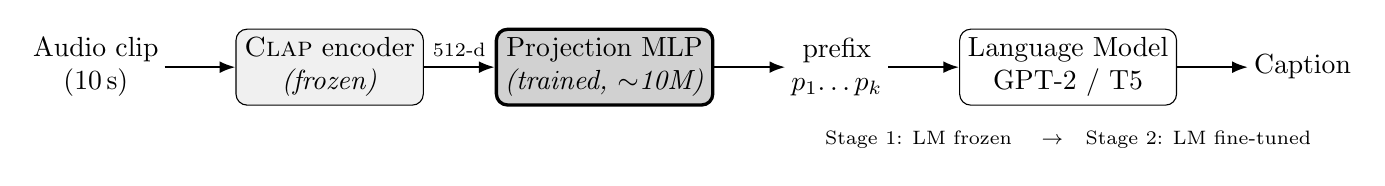
\begin{tikzpicture}[
    node distance=6mm and 9mm,
    box/.style={draw, rounded corners, minimum height=9mm, align=center, inner sep=3pt},
    frozen/.style={box, fill=black!6},
    trained/.style={box, fill=black!18, very thick},
    data/.style={align=center, inner sep=2pt},
    flow/.style={-{Latex[length=2mm]}, thick}]
  \node[data] (audio) {Audio clip\\(10\,s)};
  \node[frozen, right=of audio] (clap) {\clapenc{} encoder\\\emph{(frozen)}};
  \node[trained, right=of clap] (proj) {Projection MLP\\\emph{(trained, $\sim$10M)}};
  \node[data, right=of proj] (prefix) {prefix\\$p_1\!\dots p_k$};
  \node[box, right=of prefix] (lm) {Language Model\\GPT-2 / T5};
  \node[data, right=of lm] (cap) {Caption};
  \draw[flow] (audio) -- (clap);
  \draw[flow] (clap) -- node[above,font=\scriptsize]{512-d} (proj);
  \draw[flow] (proj) -- (prefix);
  \draw[flow] (prefix) -- (lm);
  \draw[flow] (lm) -- (cap);
  \node[font=\scriptsize, below=2mm of lm, align=center] (s) {Stage~1: LM frozen \quad$\rightarrow$\quad Stage~2: LM fine-tuned};
\end{tikzpicture}
\caption{The \sys{} pipeline. A frozen \clapenc{} encoder turns the audio clip into a single
512-d embedding; a small projection MLP (the only newly added module) maps it to a $k$-token
prefix in the LM embedding space; the LM generates the caption. Stage~1 trains the projection
with the LM frozen; Stage~2 additionally fine-tunes the LM.}
\label{fig:pipeline}
\end{figure}

\section{Audio encoder}
We use the LAION \clapenc{} checkpoint \texttt{laion/clap-htsat-unfused}~\cite{wu2023clap},
whose audio tower is an HTS-AT transformer~\cite{chen2022htsat} producing a $512$-dimensional
audio embedding. \clapenc{} is trained on general audio and is \emph{not}
music-specialised --- a deliberate test of how far a general frontend carries on a music task.
We additionally benchmark this general frontend against music-specialised encoders as a second
ablation axis (Section~\ref{sec:encoder}). Embeddings are precomputed once and cached, so the
encoder never runs during training or evaluation. The ``unfused'' variant ingests a fixed
$\sim$10\,s window, matching MusicCaps clip length.

\section{Projection network}
The projection is a small MLP,
$\text{Linear}\!\rightarrow\!\text{LayerNorm}\!\rightarrow\!\text{GELU}\!\rightarrow\!
\text{Dropout}\!\rightarrow\!\text{Linear}$, reshaped to $(k,d_{\text{lm}})$. The baseline uses
prefix length $k{=}8$, dropout $0.3$ and depth $2$.

\section{Language models}
We compare GPT-2~\cite{radford2019gpt2} (decoder-only, 124M) and T5-base~\cite{raffel2020t5}
(encoder--decoder, 220M). For T5 the prefix is fed to the encoder; for GPT-2 it is prepended as
input embeddings. Extending the same harness to modern billion-parameter decoders is in progress
(Chapter~\ref{ch:conclusion}).

\section{Two-stage training}
In Stage~1 (S1) the LM is frozen and only the projection is trained; in Stage~2 (S2) the
projection and the full LM are fine-tuned together (the audio encoder stays frozen). S1
corresponds to ClipCap's frozen-LM regime and S2 to its fine-tuned-LM regime. The objective in
both stages is autoregressive cross-entropy on caption tokens conditioned on the prefix,
\[
  \mathcal{L} = -\sum_{j}\log p_\theta\!\left(c_j \mid p_1,\dots,p_k, c_1,\dots,c_{j-1}\right).
\]
We use AdamW~\cite{loshchilov2019adamw} (weight decay $0.1$), cosine
annealing~\cite{loshchilov2017sgdr}, batch size $8$ and early stopping
(patience $5$). Per model, only the learning rates are tuned, via a 16-trial
Optuna~\cite{akiba2019optuna} search over an 8-epoch proxy; all else is fixed so the LM stays
the controlled variable.

\section{Efficiency}
The only newly added module is the projection ($\sim$$10.2$M parameters): Stage~1 trains it
alone with the LM frozen, and Stage~2 additionally fine-tunes the LM. The complete model is
$124$M (GPT-2) or $220$M (T5) parameters --- one to two orders of magnitude smaller than the
billion-parameter end-to-end audio LLMs --- and every experiment in this report runs on a
single consumer GPU (NVIDIA RTX~5090). Because \clapenc{} embeddings are precomputed once,
the audio encoder is never run during training.

%---------------------- Experimental Study ----------------------%
\chapter{EXPERIMENTAL STUDY}\label{ch:experiments}

\section{Experimental setup}

\textbf{Test environment.}
All experiments run on a single workstation with an NVIDIA RTX~5090 GPU. The software stack is
Python with PyTorch and the HuggingFace \texttt{transformers} library for the models, Optuna
for hyperparameter search, and the \texttt{aac-metrics} package (with a Java runtime for its
CoreNLP-backed metrics) for evaluation.

\textbf{Data.}
We use MusicCaps~\cite{agostinelli2023musiclm} with a fixed three-way random split: a held-out
test set ($n{=}529$, final metrics only), a validation set ($n{\approx}495$, for checkpoint
selection and hyperparameter search), and the remainder for training ($n{\approx}4{,}455$). The
split seed is fixed across all conditions, so every model and seed is scored on the identical
test set.

\textbf{Metrics.}
A single shared harness scores all conditions with the \texttt{aac-metrics} suite: BLEU-1 and
BLEU-4~\cite{papineni2002bleu}, METEOR~\cite{banerjee2005meteor}, ROUGE-L~\cite{lin2004rouge},
CIDEr-D~\cite{vedantam2015cider}, SPICE~\cite{anderson2016spice}, SPIDEr~\cite{liu2017spider},
SBERT-sim, FER and \fense{}.
\fense{}~\cite{zhou2022fense} is our primary metric: it combines a
Sentence-BERT~\cite{reimers2019sbert} semantic similarity with a fluency-error penalty (FER),
making it sensitive to the semantic correctness a listener cares about. We apply no
post-processing by default; sentence trimming is treated as an explicit decoding ablation
(Section~\ref{sec:decoding}).

\textbf{Noise floor.}
To judge whether a delta is real, we retrain each baseline with three seeds (42,\,43,\,44),
varying only initialisation, shuffling and dropout while holding the data split fixed. The
standard deviation of each metric across seeds is our \emph{noise floor}; deltas smaller than it
are not interpreted as effects.

\section{Baseline comparison}\label{sec:baseline}
Figure~\ref{fig:baseline_groups} reports greedy-decoding test metrics with per-model noise
floors, split into the \textbf{Legacy metrics} and \textbf{AAC metrics} groups following the
\texttt{aac-metrics} taxonomy --- the two groups live on different scales, so separate panels
let each be inspected at its own resolution (exact values in Tables~\ref{tab:baseline_legacy}
and~\ref{tab:baseline_aac} in the appendix). GPT-2 leads on nine of the ten metrics,
including the primary \fense{} ($0.3998$ vs.\ $0.3954$); the exception is FER, where T5 is
lower (better), though that gap ($0.023$) sits inside T5's own FER noise floor ($\pm0.0511$).
The \fense{} margin ($0.004$) is likewise smaller than either
model's \fense{} noise floor ($\pm0.0137$ for GPT-2, $\pm0.0345$ for T5). We therefore do
\emph{not} read it as evidence that one architecture is better at music captioning under this
recipe. The noise floor is also $\sim$$2.5\times$ larger for T5 than GPT-2, so the
encoder--decoder is noticeably noisier run-to-run and each model must be judged against its
\emph{own} variance.

\begin{figure}[htbp]\centering
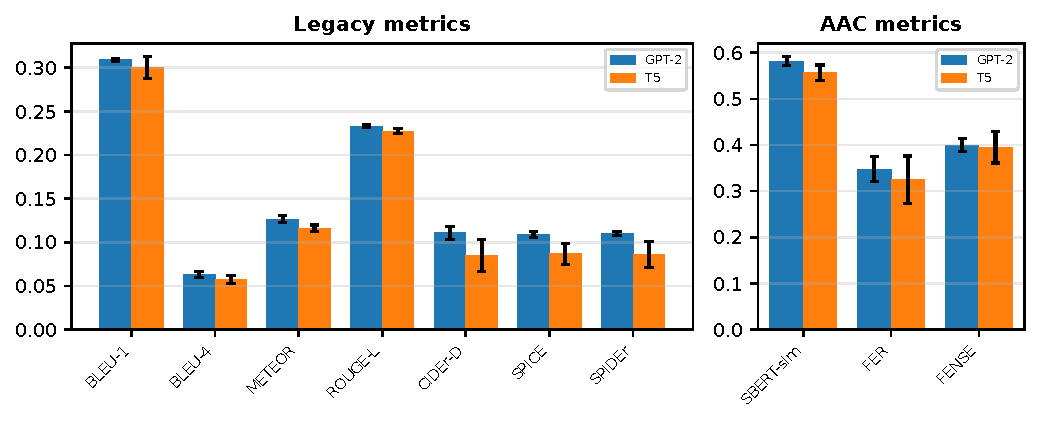
\includegraphics[width=\textwidth]{figures/fig_baseline_groups.pdf}
\caption{Baseline (greedy) test-set metrics per model, grouped into
\textbf{Legacy metrics} (left) and \textbf{AAC metrics} (right), each panel at
its own scale. Error bars show the per-model run-to-run standard deviation
(noise floor) where measured. All metrics are higher-is-better except FER
(lower is better).}
\label{fig:baseline_groups}
\end{figure}

\FloatBarrier
\section{Stage~1 vs.\ Stage~2}\label{sec:stages}
Figure~\ref{fig:training} shows validation loss per epoch for every projection configuration,
and Table~\ref{tab:spread_collapse} summarises the per-configuration best values. In Stage~1,
where only the projection is trained, the configurations spread widely (a range of
$0.38$ for GPT-2 and $0.83$ for T5). After Stage~2 fine-tuning that spread collapses to $0.03$
for both models --- an $11\times$ reduction for GPT-2 and $31\times$ for T5: full fine-tuning
largely erases the architectural differences introduced by the
projection. The S2 curves also reveal early overfitting --- validation loss bottoms within a few
epochs and then rises --- which early stopping handles.

\begin{table}[ht]
\centering
\caption{Best validation loss per configuration at Stage~1 (projection only) and Stage~2 (full fine-tuning). The spread row shows the S1 spread collapsing after S2 fine-tuning (GPT-2 11$\times$, T5 31$\times$).}
\label{tab:spread_collapse}
\footnotesize
\resizebox{\ifdim\width>\linewidth\linewidth\else\width\fi}{!}{%
\begin{tabular}{lrrrr}
\toprule
Config & GPT-2 S1 & GPT-2 S2 & T5 S1 & T5 S2 \\
\midrule
baseline & 2.6480 & 2.0573 & 2.4293 & 1.8903 \\
depth1 & 2.8870 & 2.0530 & 3.0239 & 1.8929 \\
depth3 & 2.6068 & 2.0609 & 2.3263 & 1.8674 \\
drop0.1 & 2.6821 & 2.0570 & 2.3150 & 1.8941 \\
drop0.5 & 2.6138 & 2.0554 & 2.2927 & 1.8855 \\
prefix16 & 2.5091 & 2.0861 & 2.1973 & 1.8793 \\
prefix4 & 2.8041 & 2.0601 & 2.4628 & 1.8900 \\
\textbf{Spread} & \textbf{0.3779} & \textbf{0.0332} & \textbf{0.8266} & \textbf{0.0267} \\
\bottomrule
\end{tabular}
}
\end{table}


\begin{figure}[t]\centering
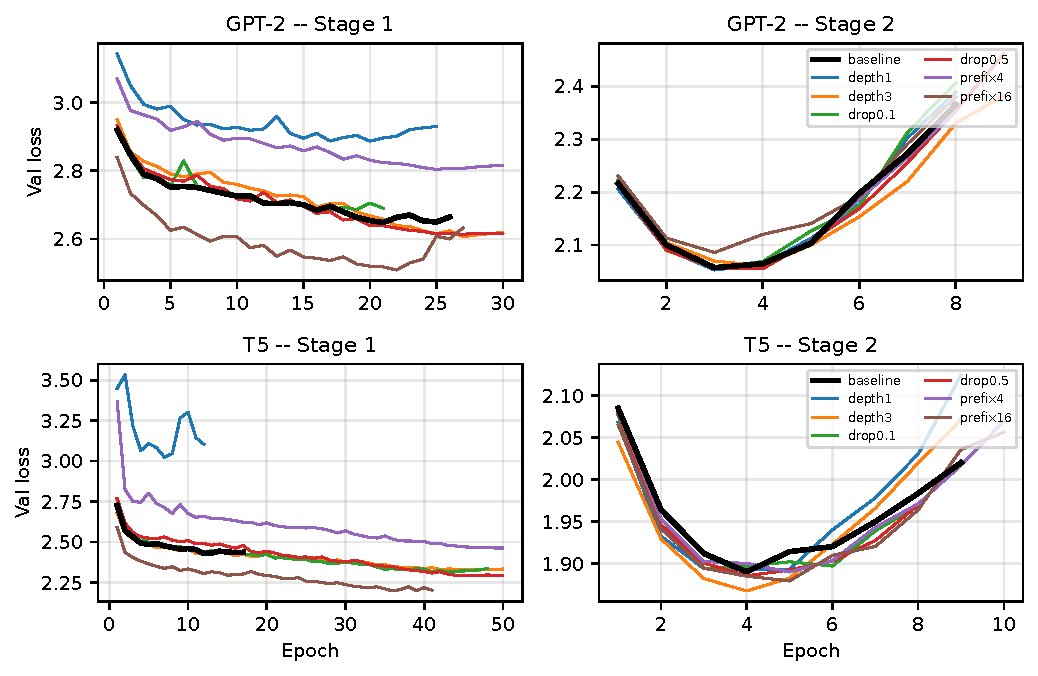
\includegraphics[width=\textwidth]{figures/fig_training_curves.pdf}
\caption{Validation loss per epoch for all projection configurations. \emph{Left:} Stage~1
(projection only) shows a wide spread across configurations. \emph{Right:} Stage~2 (full
fine-tuning) collapses that spread --- the configurations become nearly indistinguishable ---
and shows the early-overfitting onset. The baseline is drawn in bold.}
\label{fig:training}
\end{figure}

\FloatBarrier
\section{Architecture ablations}\label{sec:arch}
We vary prefix length ($\{4,16\}$ around $8$), dropout ($\{0.1,0.5\}$ around $0.3$) and
projection depth ($\{1,3\}$ around $2$), retraining each from scratch with greedy decoding.
Figure~\ref{fig:arch} plots the resulting \fense{} against the baseline $\pm$ noise-floor band.
Consistent with Section~\ref{sec:stages}, most configurations fall within the band: no projection
hyperparameter reliably moves the primary metric for GPT-2. For T5 the prefix variants produce
larger \fense{} swings, but --- as the next section shows --- these coincide with collapses in
the fluency-error term rather than genuine semantic gains. Full per-configuration metric tables
are given in the appendix.

\begin{figure}[t]\centering
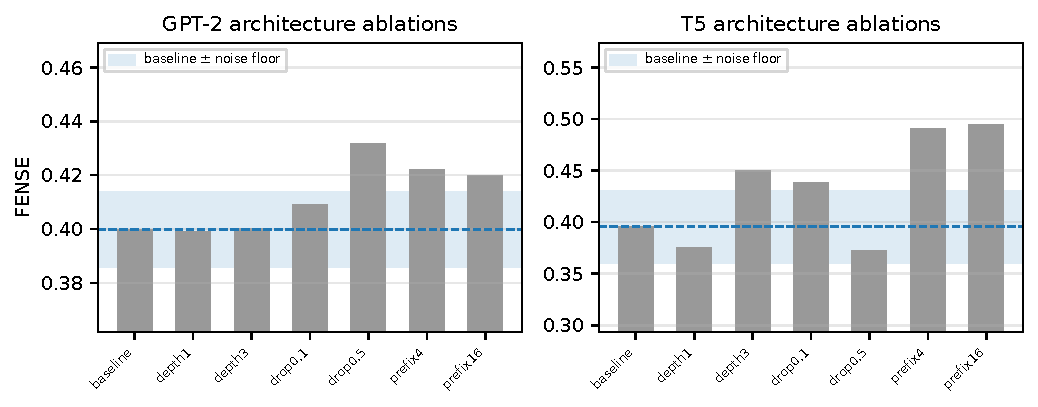
\includegraphics[width=\textwidth]{figures/fig_arch_noisefloor.pdf}
\caption{Architecture-ablation \fense{} per configuration. The shaded band is the baseline
$\pm$ one noise-floor standard deviation. Bars inside the band are not distinguishable from the
baseline.}
\label{fig:arch}
\end{figure}

\FloatBarrier
\section{Decoding ablations}\label{sec:decoding}
Decoding strategies are evaluated on the fixed baseline checkpoint (no retraining), isolating
generation behaviour. Figure~\ref{fig:decoding_groups} shows the top configurations by
\fense{} per model, split into \textbf{Legacy metrics}, \textbf{AAC metrics} and a separate
FER panel so each group can be read at its own resolution (full tables in the appendix,
Tables~\ref{tab:decoding_gpt2_legacy}--\ref{tab:decoding_t5_aac}). The dominant lever is
trimming trailing incomplete sentences: it lifts \fense{} from $0.3998$ to $0.5796$ for GPT-2
and from $0.3954$ to $0.5762$ for T5.

This gain is, however, \emph{largely an artifact of the metric}. Figure~\ref{fig:fensefer} plots
\fense{} against FER across all decoding configurations: the relationship is almost perfectly
inverse, and the trimmed configurations simply drive FER to near zero while the lexical metrics
in Tables~\ref{tab:decoding_gpt2_legacy} and~\ref{tab:decoding_t5_legacy} barely move. In
other words, trimming removes the
fluency penalty inside \fense{} without making captions semantically more correct. We report it
as a useful decoding choice for producing clean captions, but caution against reading the
headline \fense{} jump as a semantic improvement.

\begin{figure}[t]\centering
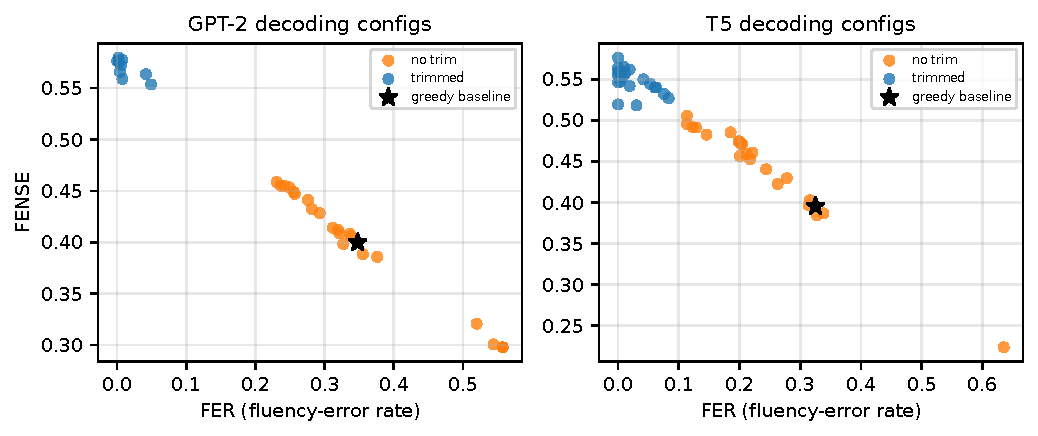
\includegraphics[width=\textwidth]{figures/fig_decoding_fense_fer.pdf}
\caption{\fense{} vs.\ FER over all decoding configurations. The near-perfect inverse trend shows
that \fense{} here is dominated by the fluency-error term: trimmed configurations (low FER) score
high \fense{} without improving semantic similarity. The star is greedy decoding.}
\label{fig:fensefer}
\end{figure}

\begin{figure}[htbp]\centering
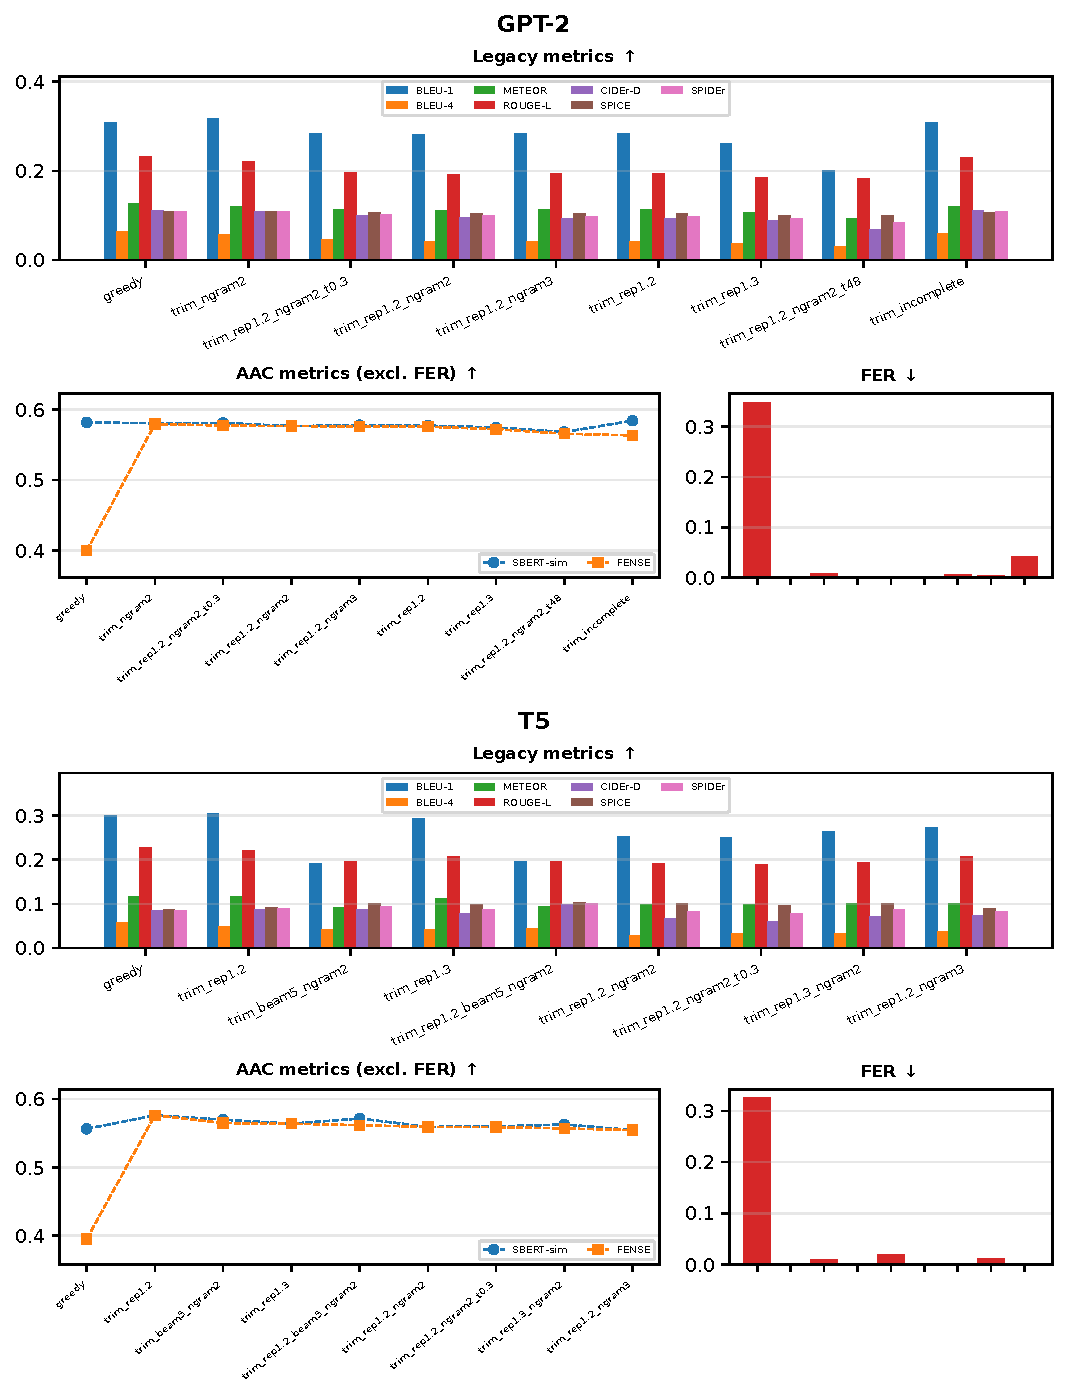
\includegraphics[width=\textwidth]{figures/fig_decoding_groups.pdf}
\caption{Decoding-ablation metrics per model (greedy baseline plus top
configurations by \fense{}). Each model section shows \textbf{Legacy metrics}
(top, full width), with \textbf{AAC metrics excluding FER} (bottom left) and
\textbf{FER} (bottom right) beneath, each panel at its own scale. The AAC panel uses markers on a zoomed (non-zero) axis to resolve the
narrow 0.55--0.58 band of the trimmed configurations; FER is separated because
its near-zero trimmed values would otherwise compress that axis, and its bars
follow the same configuration order as the adjacent panel. The flat SBERT-sim
trace next to the jumping \fense{} trace and collapsing FER bars visualises
the trimming artifact of Figure~\ref{fig:fensefer}.}
\label{fig:decoding_groups}
\end{figure}

\FloatBarrier
\section{Audio-encoder ablation}\label{sec:encoder}
The experiments so far hold the audio frontend fixed and vary the language model. The second
axis of this study does the reverse: it keeps the language model fixed (GPT-2, the cheaper of
the two) and swaps the frozen \clapenc{} encoder for music-specialised alternatives,
re-extracting the cached embeddings and re-running the learning-rate search per encoder while
leaving the projection, training protocol and evaluation untouched. Because second-stage
fine-tuning was shown above to erase upstream differences (Section~\ref{sec:stages}), we run
this comparison at Stage~1 (projection only, LM frozen), where the frontend signal is most
exposed, and replicate every encoder over the three noise-floor seeds.

We compare the general-audio baseline \texttt{clap-htsat-unfused} against two music \clapenc{}
checkpoints (\texttt{larger\_clap\_music}, \texttt{larger\_clap\_music\_and\_speech}), two MERT
variants (95M, 330M)~\cite{li2024mert}, MusicFM~\cite{won2024musicfm}, and the 2025
self-supervised models MuQ and MuQ-MuLan~\cite{zhu2025muq}.
Figure~\ref{fig:encoder} reports per-encoder \fense{} (mean over three seeds) against the
baseline $\pm$ noise-floor band. Only two encoders clear the band (mean$-$std above
baseline$+$std): \texttt{clap-music-speech} ($0.325\pm0.027$) and \texttt{muq-mulan}
($0.321\pm0.008$), against the general baseline ($0.264\pm0.018$). The remaining five sit
inside the band and are not separable from general \clapenc{} at this stage --- including the
frame-level self-supervised encoders MERT, MusicFM and MuQ, the last of which leads the
MARBLE music-understanding benchmark yet does not separate here. The signal that survives is
therefore the \emph{pooled joint audio--text} pretraining shared by the two clearers (a music
CLAP and MuQ-MuLan), not raw self-supervised acoustic features: at the frozen-projection stage a
CLAP-style clip embedding is what the projection can exploit. The wide S1 noise floor (some
encoders $\pm0.03$--$0.05$) is consistent with Stage~1 being the noisier regime, so only the two
clearers are defensible as ``meaningful differences''. The encoder learning-rate sweeps are in
the appendix (Figure~\ref{fig:lrsearch_enc}).

\begin{figure}[htbp]\centering
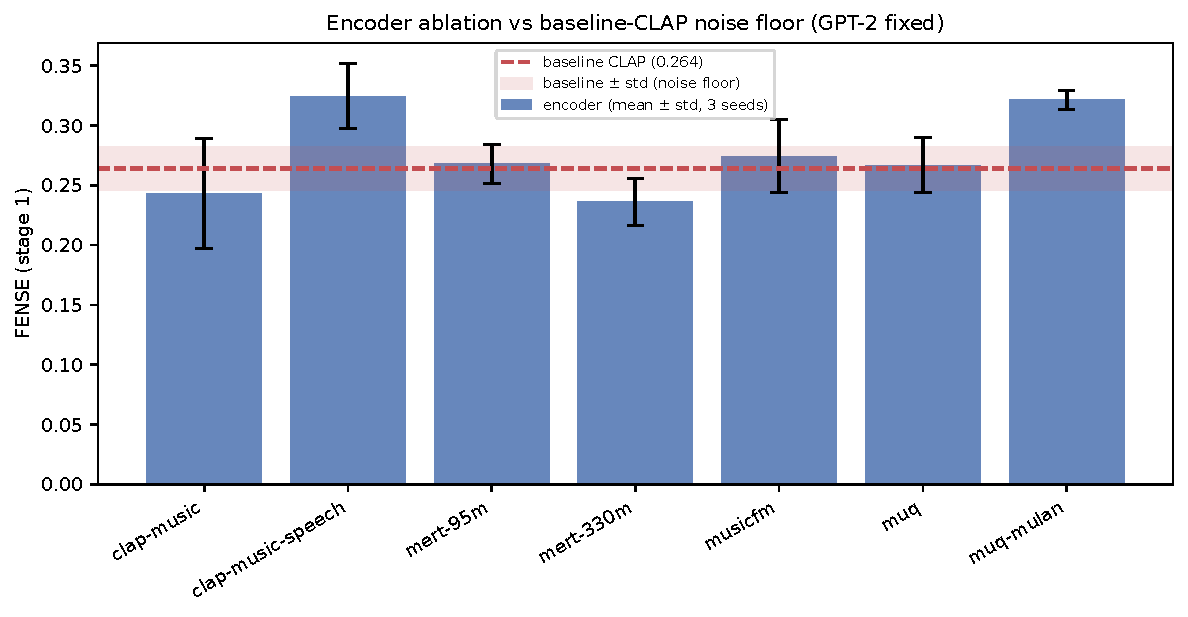
\includegraphics[width=\textwidth]{figures/fig_encoder_noisefloor.pdf}
\caption{Audio-encoder ablation: Stage-1 \fense{} per encoder (mean over three seeds, error
bars one standard deviation) with GPT-2 fixed. The shaded band is the general-\clapenc{}
baseline $\pm$ one noise-floor standard deviation; only \texttt{clap-music-speech} and
\texttt{muq-mulan} clear it.}
\label{fig:encoder}
\end{figure}

\FloatBarrier
\section{Qualitative analysis}\label{sec:qual}
Table~\ref{tab:qual} shows representative successes and failures. The models reliably recover
high-level musical content --- genre (rock, jazz, electronic), instrumentation (electric guitar,
bass, drums, piano) and mood (groovy, energetic, emotional). Two failure modes recur: on
\emph{non-music} audio the pipeline still emits a confident music caption, and greedy decoding
occasionally degenerates into verbatim repetition. Notably, degeneration and semantic accuracy
co-occur: in the bowl-tone example both models correctly capture the sound itself --- a
resonating bowl, rubbed or struck, with a meditative mood --- yet both repeat themselves, T5
collapsing into the same sentence four times over and GPT-2 duplicating its final sentence.
On non-music audio the spurious male vocalist appears only in GPT-2's printer caption; T5
instead invents a plausible non-vocal scene (a DJ scratching). Most strikingly, both models tend to insert
``a male vocalist singing melodically'' even when the reference explicitly states there is no
singer.

To characterise this we measured vocal-presence and vocalist-gender agreement over the full
test set (full statistics in Tables~\ref{tab:vocal_bias} and~\ref{tab:vocal_bias_context} in
the appendix). The bias is \emph{not} a blind spot: GPT-2 mentions vocals on 95\% of clips whose
reference describes singing, but also on 43\% of clips marked instrumental (T5: 82\%\,/\,29\%)
--- both models track vocal presence well above chance while skewing toward false positives.
The skew mirrors the training captions, of which 53\% mention vocals and in which male
vocalists outnumber female ones 2.2:1; the phrase ``male vocalist'' appears in 10\% of training
captions but in roughly half of the generated ones. Gender is worse: on references describing a
\emph{female} singer, T5 outputs ``male'' 89\% of the time and GPT-2 44\%, while male
references are almost never misgendered (2--4\%). These rates persist across decoding
configurations, so they are not a decoding artifact.

To separate the frontend from the LM, we probed the frozen \clapenc{} embeddings directly with
zero-shot text prompts: vocal vs.\ instrumental is separable at 74\% accuracy and vocalist
gender at 76\% (female recall only 55\%). The embedding therefore carries the relevant cues,
but noisily --- and since both LMs read the \emph{same} embedding, the gap between GPT-2
(56\%) and T5 (11\%) in female-vocalist accuracy shows the failure is largely model-side. We
conclude that the vocalist bias is caption-prior amplification under uncertain audio evidence,
not a missing audio cue: a music-specialised encoder should sharpen the evidence, but the
male-vocalist default itself is learned from the caption statistics.

\begin{table*}[t]
\centering
\footnotesize
\caption{Representative successes and failures (baseline greedy; captions trimmed at the last full sentence for display). The models recover genre, instrumentation and mood, but default to a male vocalist even on instrumental or non-music audio.}
\label{tab:qual}
\begin{tabularx}{\textwidth}{lX}
\toprule
\multicolumn{2}{c}{\textbf{Successes}}\\
\midrule
\addlinespace[2pt]
\emph{Reference} & instrumental rock music with a drum kit, lots of cymbal crashes, acoustic guitar strumming, harmonized lead guitars and an active bass guitar. \\
\emph{GPT-2} & This is a rock music piece. There is a male vocalist singing melodically. The electric guitar is playing the main tune while the bass guitar is playing in the background. The rhythmic background consists of a simple acoustic drum beat. The atmosphere is groovy. \\
\emph{T5} & This is a rock music piece. There is a male vocalist singing melodically. The electric guitar is playing a simple tune with a bass guitar playing in the background. The rhythmic background consists of a fast-paced acoustic drum beat. \\
\midrule
\addlinespace[2pt]
\emph{Reference} & This is a drum \& bass electronic music piece. There is no singer. There is a strong and fuzzy feeling bass sound. The rhythmic background consists of a loud and high tempo electronic drum beat. The atmosphere is modern and energetic. This piece could be playing at a nightclub or a dance club. \\
\emph{GPT-2} & This is a techno music piece. There is a male vocalist singing melodically. The melody is being played by the synth bass. The rhythmic background consists of a fast-paced electronic drum beat. The atmosphere is groovy. This piece could be used in the background of nightclubs. \\
\emph{T5} & This is a techno house music piece. There is a male vocalist singing melodically. The melody is being played by the synth bass while the rhythmic background consists of a fast-paced electronic drum beat. The atmosphere is energetic. \\
\midrule
\addlinespace[2pt]
\emph{Reference} & A female vocalist sings this melancholic melody in a foreign language. The tempo is slow with a romantic piano accompaniment. The song is soft, mellow, poignant, emotional, sentimental, romantic, melancholic, sad, lonely, and wistful. This song is a Pop/ Love song. \\
\emph{GPT-2} & This is a lullaby piece. There is a female vocalist singing melodically. The piano is playing a simple tune while the bass guitar is playing in the background. The atmosphere is calming and relaxing. This piece could be used in the background of a meditation video. \\
\emph{T5} & This is a classical music piece. There is a female vocalist singing melodically. The melody is being played by the piano while the rhythm is being played by the acoustic guitar. The atmosphere is romantic. \\
\midrule
\addlinespace[2pt]
\emph{Reference} & The low quality recording features a live performance of a jazz song and it consists of a groovy bass guitar, groovy rhodes keys, electric guitar melody, shimmering hi hats, punchy kick and punchy snare hits. It sounds groovy, funky and passionate. The recording is noisy and in mono. \\
\emph{GPT-2} & This is a jazz music piece. There is a saxophone solo being played. The melody is being played by the piano and the electric guitar. The rhythmic background consists of a simple acoustic drum beat. The atmosphere is groovy. This piece could be used in the background of a jazz bar. \\
\emph{T5} & This is a live recording of a jazz music piece. There is a saxophone playing the lead melody while a bass guitar is playing in the background. The rhythm is being played by the acoustic drums. The atmosphere is jazzy. \\
\midrule
\multicolumn{2}{c}{\textbf{Failure cases}}\\
\midrule
\addlinespace[2pt]
\emph{Reference} & The low quality recording features a printer that produces printing sounds and some muffled music playing in the background, probably on a radio. It is noisy and in mono. \\
\emph{GPT-2} & This is a recording of a live performance of a pop music piece. There is a male vocalist singing melodically. The melody is being played by a keyboard and a bass guitar while the rhythmic background is provided by a fast tempo electronic drum beat. \\
\emph{T5} & This is a live recording of a DJ performance. The DJ is scratching the turntable repeatedly. The turntable is a low quality recording. The sound of the turntable is distorted and the recording is of very poor quality. \\
\midrule
\addlinespace[2pt]
\emph{Reference} & The low quality recording features a metallic hit, followed by resonating bowl tone. The recording is mono and noisy. \\
\emph{GPT-2} & This is a meditation music piece. There is a bowl-like sound being played by the bowl. The bowl is being rubbed repeatedly. There is a calming and relaxing atmosphere to this piece. This piece can be used in the background of meditation videos. It can also be used in the background of meditation videos. \\
\emph{T5} & This is a Tibetan singing bowl playing in the background of a meditation video. There is a chanting bowl being played. There is a chanting bowl being played. There is a chanting bowl being played. There is a chanting bowl being played. \\
\bottomrule
\end{tabularx}
\end{table*}


\FloatBarrier
\section{Comparison with reference captioners}\label{sec:reference}
To place the pipeline against existing systems without the invalid cross-dataset comparison of
Chapter~\ref{ch:related}, we score a set of zero-shot reference captioners on the \emph{same}
MusicCaps test split through the same metric harness. These models ingest raw audio and bypass
the \clapenc{}--projection--LM design, so they are an external reference, not controlled ablation
rows. They span general audio-LMs --- Audio Flamingo (the AF-Next captioner
checkpoint)~\cite{ghosh2026afnext}, Qwen2-Audio~\cite{chu2024qwen2audio} and a Qwen3-Omni
captioner~\cite{xu2025qwen3omni} --- and
music-domain captioners --- LP-MusicCaps~\cite{doh2023lpmusiccaps} and
BLAP~\cite{lanzendorfer2025blap}. Figure~\ref{fig:reference_fense} summarises the primary
metric and Figures~\ref{fig:ref_music} and~\ref{fig:ref_general} give the per-metric
breakdown, with full values in Table~\ref{tab:reference-comparison} in the appendix.

Leakage is the central caveat. Several references may have seen MusicCaps in training:
Qwen2-Audio attains the highest \fense{} ($0.665$) but \emph{sweeps every metric including the
lexical ones}, the signature of training on the target captions; the MusicCaps-fine-tuned
LP-MusicCaps (transfer) reaches \fense{} $0.702$ with a CIDEr-D of $3.733$ --- an order of
magnitude above any honest row --- which is train-on-test memorisation, since ${\sim}48\%$ of
our random test split falls in its official-train set. We mark such rows with a dagger and,
where a model was fine-tuned on MusicCaps-train, additionally report a leakage-free
\emph{held-out} score on the MusicCaps-official-eval subset ($n{=}284$).

Among \emph{leakage-free} rows the lightweight pipeline is competitive: GPT-2 at its best
decoding configuration reaches \fense{} $0.580$, the highest non-leaked score in the table,
ahead of every clean reference --- the music-domain LP-MusicCaps (pretrain, MSD-only) at
$0.378$, BLAP held-out at $0.476$, and LP-MusicCaps transfer held-out at $0.543$. The general
audio-LMs are fluent but off-style: Audio Flamingo scores well on semantics (\fense{} $0.440$,
SBERT-sim $0.586$) yet loses every lexical metric to the trained pipeline, and the 30B
Qwen3-Omni captioner is the weakest reference (\fense{} $0.396$). The reading is consistent with
the framing of this report: a small model trained on-target matches the MusicCaps caption style
that large zero-shot models miss, and only models that have arguably seen the data score clearly
higher.

\begin{figure}[htbp]\centering
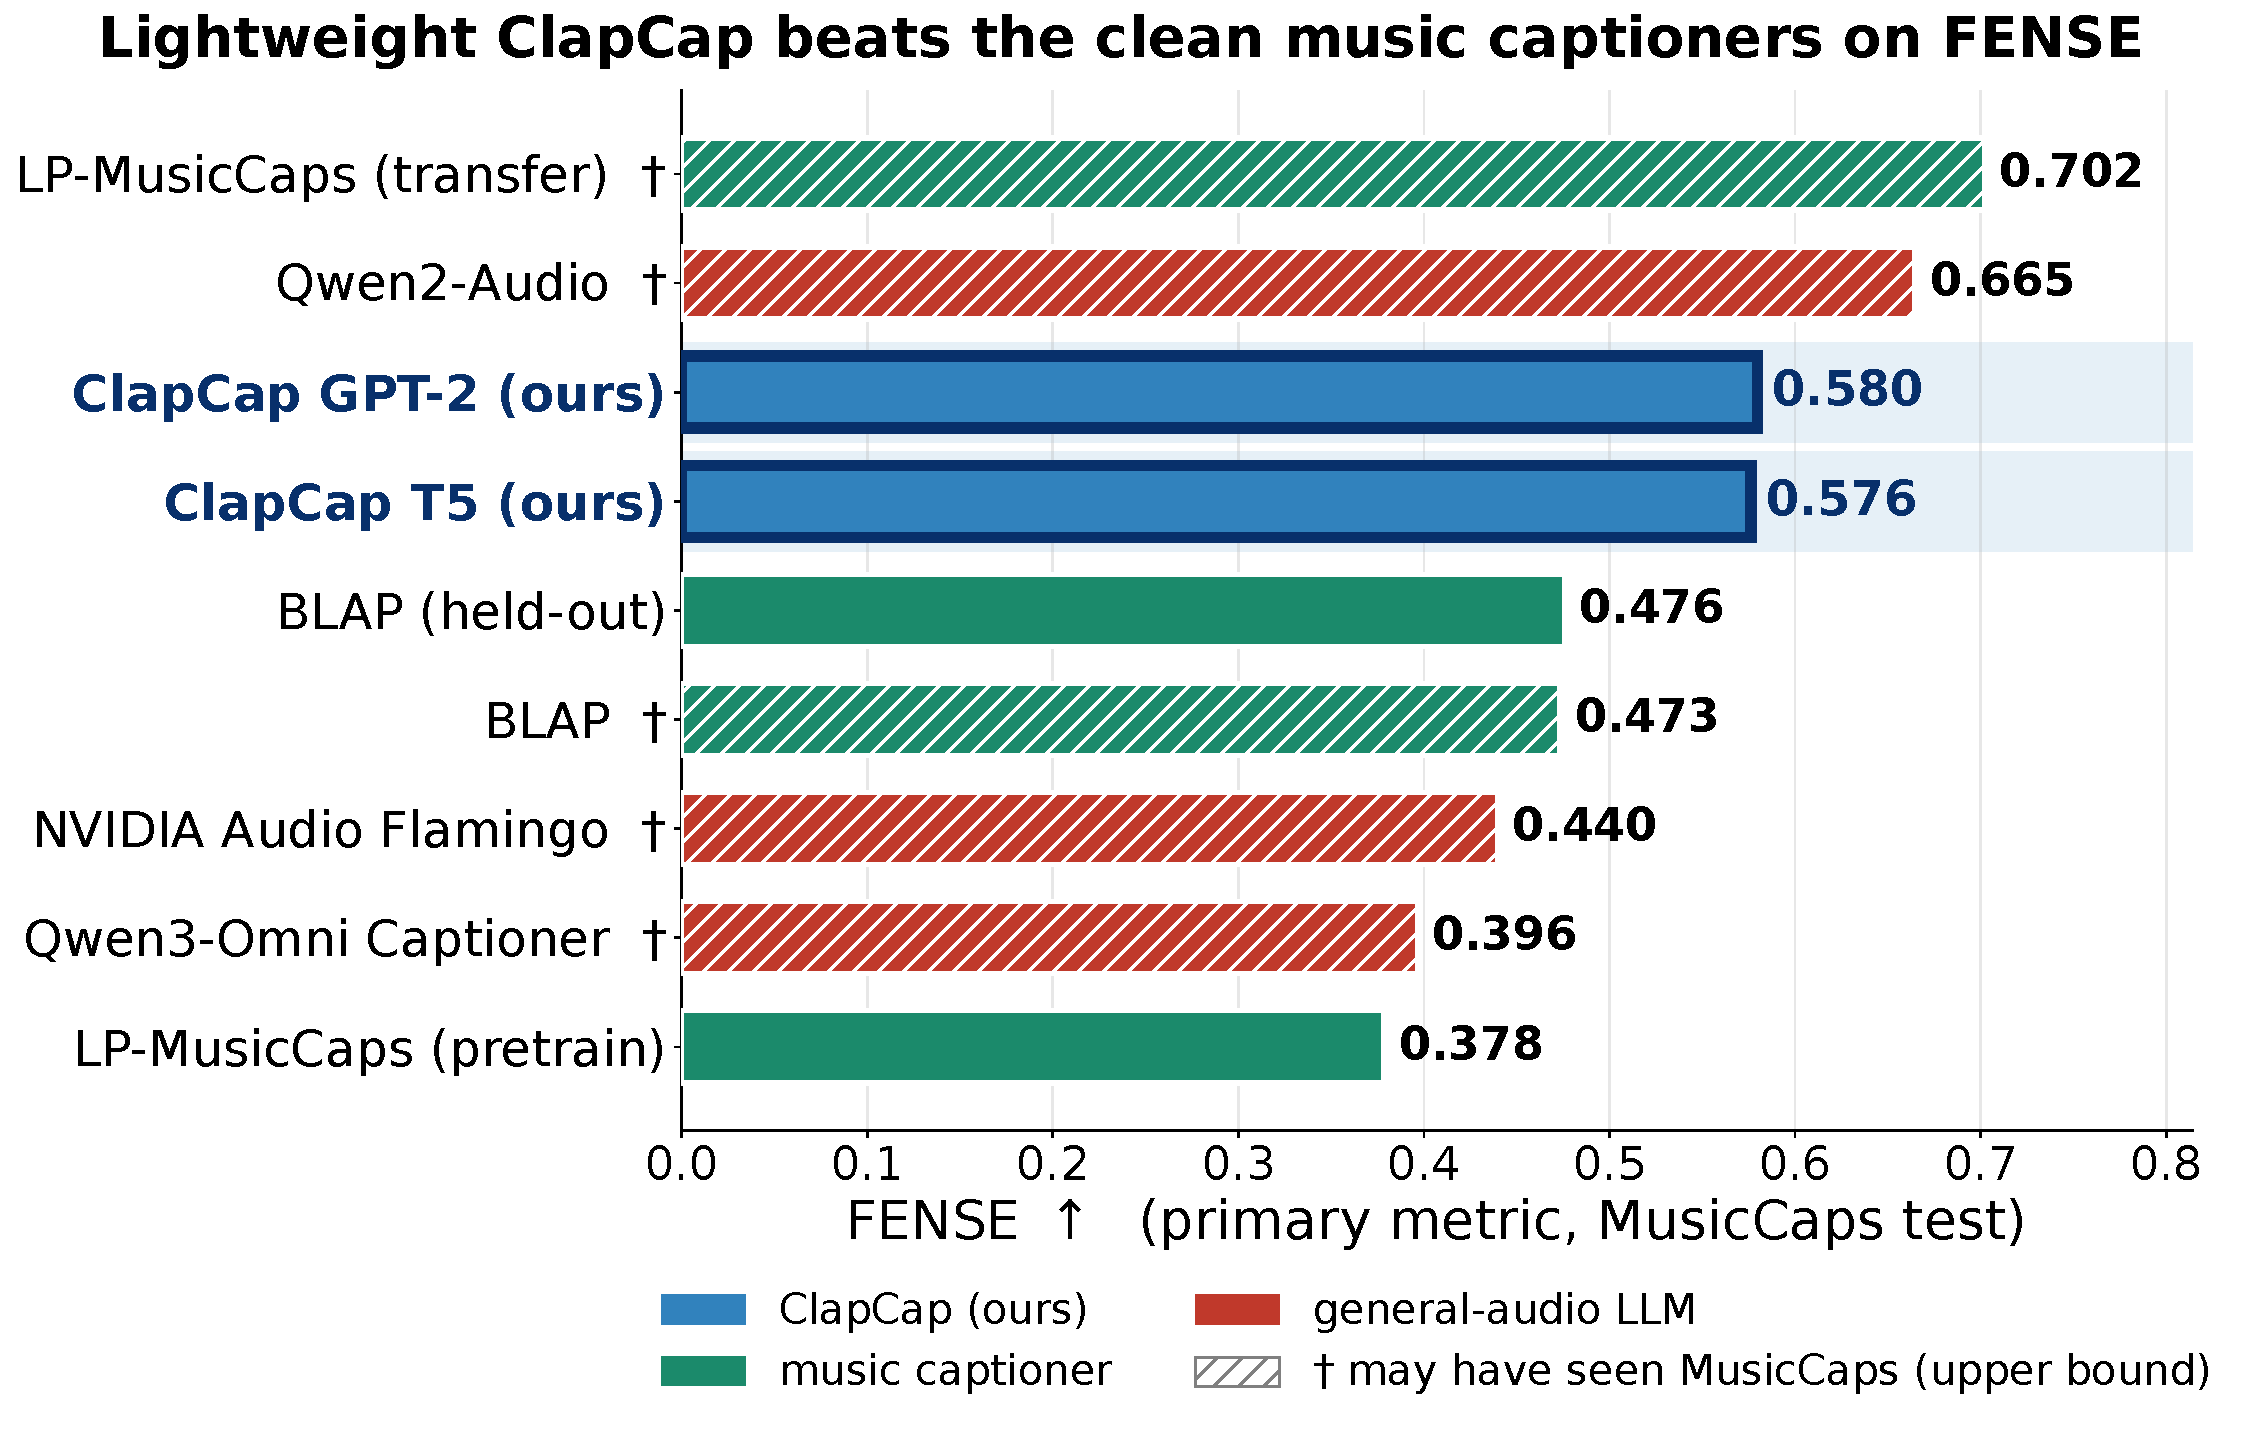
\includegraphics[width=\textwidth]{figures/fig_poster_fense.pdf}
\caption{Primary metric (\fense{}) on the shared MusicCaps test split: our lightweight
pipeline (GPT-2/T5, highlighted) against the zero-shot reference captioners. Hatched,
daggered bars may have seen MusicCaps in training (leakage upper bounds); for the two leaky
music captioners the clean held-out number is plotted instead. The pipeline's best decoding
configuration is the strongest leakage-free system. Per-metric breakdowns follow in
Figures~\ref{fig:ref_music} and~\ref{fig:ref_general}.}
\label{fig:reference_fense}
\end{figure}

\begin{figure}[htbp]\centering
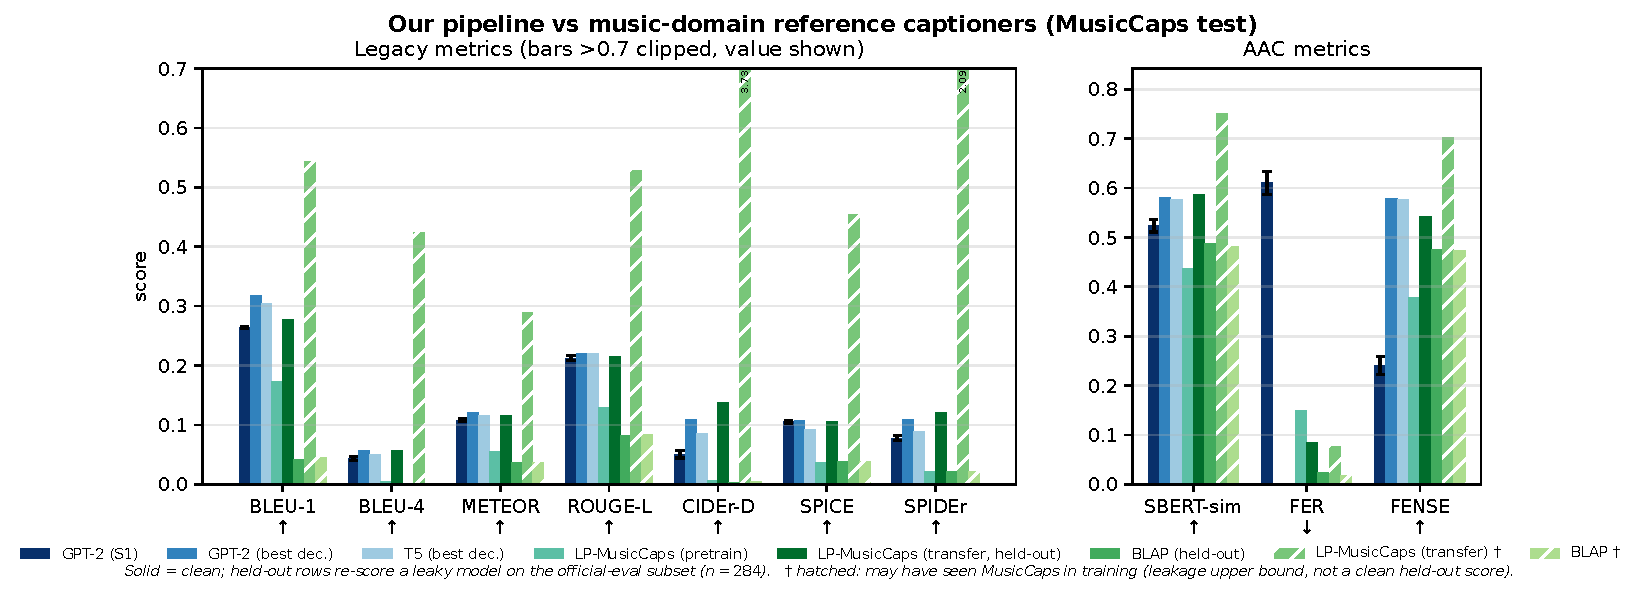
\includegraphics[width=\textwidth]{figures/fig_reference_comparison_music.pdf}
\caption{Music-domain references against the pipeline on the shared test split. Leaky rows
(hatched, daggered) are shown next to their leakage-free held-out twins so the
CIDEr-D/SPIDEr inflation is visible beside the honest numbers. Bars above the panel cap are
clipped and annotated with their true value.}
\label{fig:ref_music}
\end{figure}

\begin{figure}[htbp]\centering
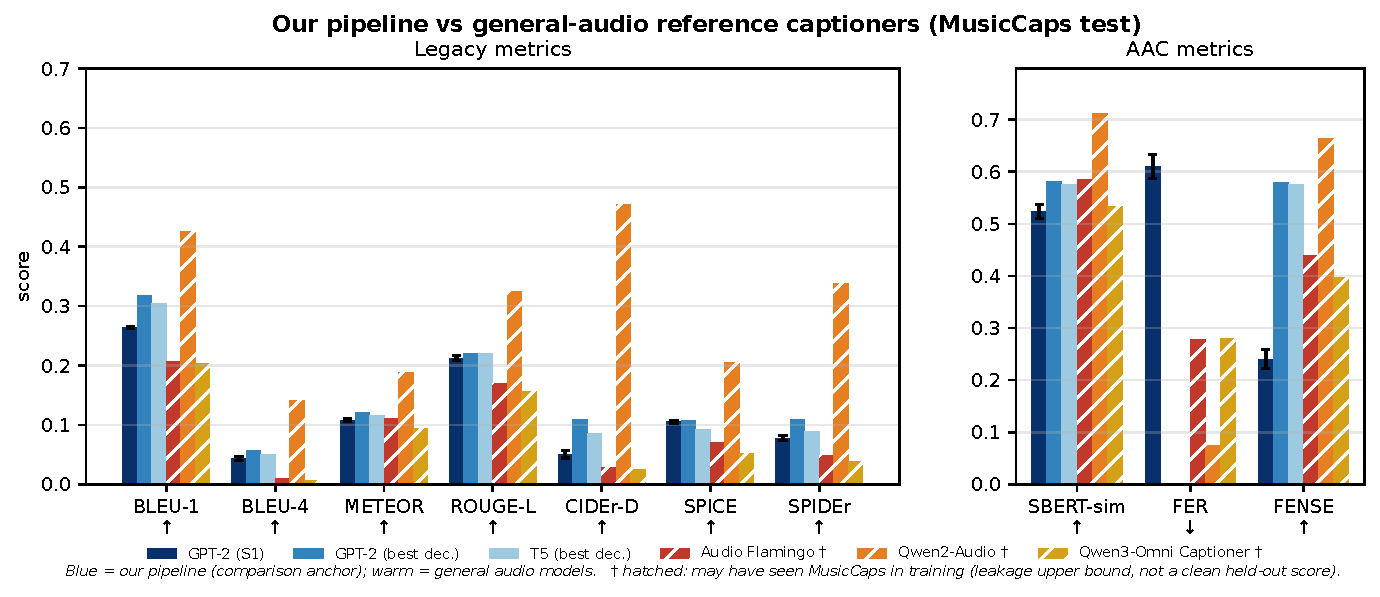
\includegraphics[width=\textwidth]{figures/fig_reference_comparison_general.pdf}
\caption{General-audio references (Audio Flamingo, Qwen2-Audio, Qwen3-Omni captioner; all
daggered as possible-leakage upper bounds) against the pipeline anchor on the shared test
split.}
\label{fig:ref_general}
\end{figure}

\FloatBarrier
\section{Human and LLM-judge evaluation}\label{sec:humaneval}
The automatic metrics rank GPT-2 and T5 as a statistical tie (Section~\ref{sec:baseline}). To
test whether that tie holds under human and model judgement --- and how far large language
models agree with people on this task --- we ran a pairwise A-vs-B study. Sixteen clip pairs
(six GPT-2-best vs.\ the human MusicCaps reference, six GPT-2-best vs.\ T5-best, four
reference-vs-mismatched-reference sanity checks) were each judged on two questions: Q1 ``which
caption is more accurate'' and Q2 ``which is less wrong'', with A/B/tie/can't-tell responses.
Pairwise comparison is used rather than absolute Likert scoring because it gives more reliable
inter-rater agreement on caption quality.

Ten lay listeners (not music experts) rated every pair; three were removed by a sanity check
(agreement with the obvious answer below $0.75$), leaving seven. The same pairs were scored by
two language-model panels under an identical rubric, both A/B orders averaged to cancel position
bias, at temperature zero with three repeats and logged model snapshots: an
\emph{audio-grounded} panel that hears the clip (Gemini~2.5~Pro, GPT-audio, Qwen3.5-Omni) and a
larger \emph{text-reference-only} panel that sees only the reference caption.

The headline is that lay raters are individually noisy but their \emph{consensus} tracks the
audio-LLM panel. Inter-human agreement is low (Fleiss $\kappa$ $0.131$ on Q1, $0.050$ on Q2),
as expected for a non-expert panel; the audio-LLM panel is more consistent ($0.392$/$0.486$).
Crucially, human-consensus versus audio-LLM-consensus agreement is substantial (Cohen $\kappa$
$0.643$ on Q1, $0.696$ on Q2; raw agreement $80\%$/$86\%$). Win-rates point the same way in
every pool (Figure~\ref{fig:winrate}): the human reference beats GPT-2 ($69\%$ of human and
$78\%$ of LLM votes prefer the reference on Q1) and GPT-2 beats T5 ($72\%$ human / $71\%$ LLM).
So the pipeline does not beat the human reference, and the \fense{} tie between GPT-2 and T5
does \emph{not} survive a preference test --- both humans and models prefer GPT-2.

Figure~\ref{fig:heatmap} shows the per-judge agreement matrix. There is no human-versus-machine
split: human consensus agrees with the GPT-audio and Qwen judges (Cohen $\kappa$ up to
$0.69$/$0.76$) more than the audio judges agree among themselves, with Gemini~2.5~Pro the
dissenting outlier. The dispersion is \emph{within} the model panel, not between humans and
models. The text-only panel is small (six GPT-2-vs-T5 pairs, directional only) and one judge
degenerates to always answering ``tie''; we report these as limitations rather than findings.

\begin{figure}[htbp]\centering
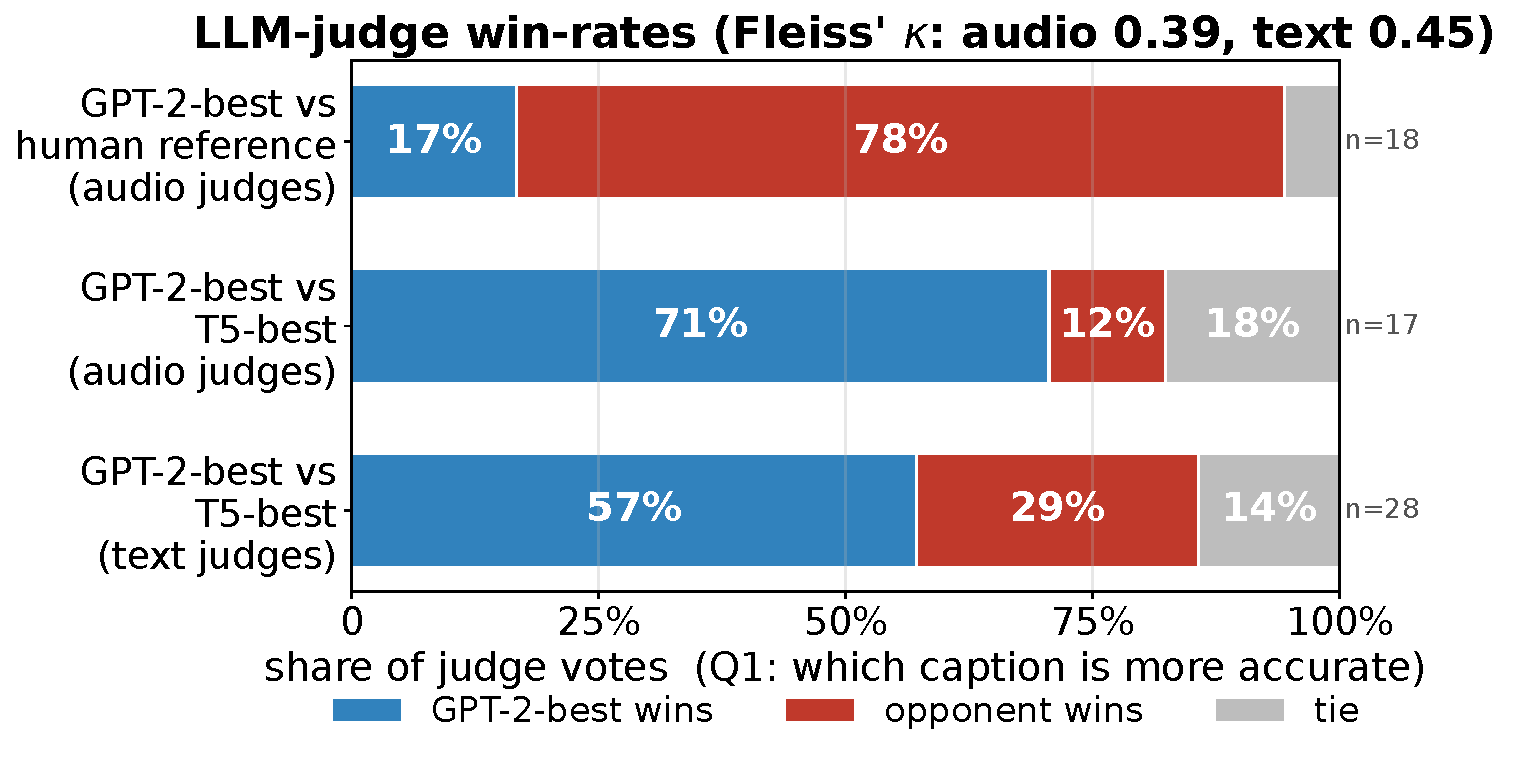
\includegraphics[width=\textwidth]{figures/fig_eval_winrate.pdf}
\caption{Pairwise A/B win-rates by rater pool. The reference-vs-GPT-2 block (the reference wins)
and the GPT-2-vs-T5 block (GPT-2 wins) point the same direction for the human, audio-LLM and
text-LLM pools. Bar counts $n$ are the decisive (non-tie) votes.}
\label{fig:winrate}
\end{figure}

\begin{figure}[htbp]\centering
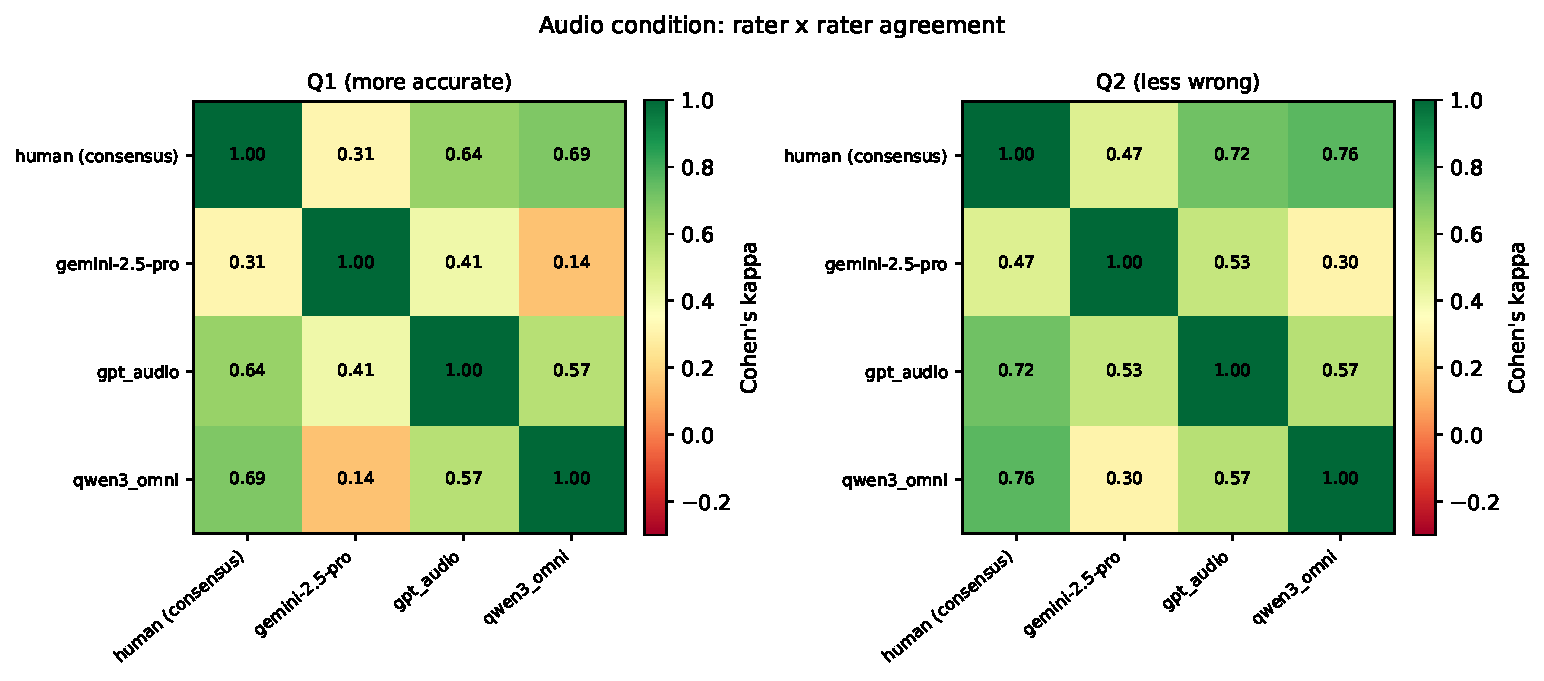
\includegraphics[width=0.8\textwidth]{figures/fig_judge_heatmap.pdf}
\caption{Per-question Cohen-$\kappa$ agreement between the human consensus and the three
audio-grounded judges. Human consensus sits with the GPT-audio and Qwen judges; Gemini~2.5~Pro
is the dissenting outlier --- the dispersion is within the model panel, not between humans and
models.}
\label{fig:heatmap}
\end{figure}

\FloatBarrier
%---------------------- Conclusions and Future Work ----------------------%
\chapter{CONCLUSIONS AND FUTURE WORK}\label{ch:conclusion}

We presented \sys{}, a controlled study of lightweight language models for \emph{music}
captioning via an audio adaptation of the ClipCap prefix recipe. Holding the frozen \clapenc{}
encoder, the projection, the data split and the evaluation fixed, we found that a decoder-only
and an encoder--decoder LM are statistically indistinguishable at baseline once run-to-run
variance is measured; that second-stage fine-tuning erases projection-level differences; and
that the largest decoding lever improves the primary metric mostly by removing a fluency penalty
rather than by improving semantics. A reproducible vocalist bias turns out to be
caption-prior amplification under uncertain audio evidence. Swapping the general frontend for
music-specialised encoders helps only marginally at the frozen-projection stage --- only pooled
audio--text encoders (a music \clapenc{} checkpoint, MuQ-MuLan) clear the noise floor, while
self-supervised acoustic encoders do not. Against zero-shot reference captioners on the same
split, the lightweight pipeline at its best decoding setting is the strongest leakage-free
system, beaten only by models that have plausibly seen MusicCaps. A pairwise human and
LLM-judge study corroborates the automatic metrics: lay-listener consensus tracks an
audio-grounded model panel, both rank the human reference above the pipeline and GPT-2 above T5,
and there is no human-versus-model split in judgement. The results characterise the minimum
viable architecture for music captioning and the care needed to interpret its metrics, rather
than chasing state of the art.

\section{Limitations}

\textbf{Audio frontend.} Our baseline encoder is trained on general audio, not music. We
benchmarked music-specialised encoders directly (Section~\ref{sec:encoder}) and found the gain
modest at the frozen-projection stage: only pooled audio--text encoders (a music \clapenc{}
checkpoint and MuQ-MuLan) clear the noise floor, while frame-level self-supervised encoders
(MERT, MusicFM, MuQ) do not separate from the general baseline. Whether a music encoder helps
more once the language model is also fine-tuned (Stage~2) is left open.

\textbf{Reference leakage.} Several of the strongest reference captioners may have been trained
on MusicCaps; we dagger them and, where possible, report leakage-free held-out scores, but their
upper-bound numbers should not be read as clean (Section~\ref{sec:reference}).

\textbf{Evaluation panel.} The human study uses ten lay listeners, not music experts, with low
individual agreement, and the text-only LLM panel covers only six pairs; the agreement results
are therefore directional and describe perceived caption quality by general listeners rather
than expert judgement.

\textbf{Capacity vs.\ data.} Scaling the LM is not free in this low-data regime
($\sim$4.5k clips). In preliminary runs a billion-parameter decoder fine-tuned end-to-end
overfits within a single epoch --- the same MLP-plus-fine-tuning overfitting that
ClipCap~\cite{mokady2021clipcap} reports, amplified by scale --- and requires a gentler schedule
to remain comparable. This supports the lightweight framing and motivates our in-progress
extension to such models.

\textbf{Metric caveats.} MusicCaps provides a single reference per clip, which mechanically
depresses n-gram metrics relative to multi-reference benchmarks. And as
Section~\ref{sec:decoding} shows, \fense{} can be inflated by fluency-driven trimming; we
mitigate this by reporting FER and lexical metrics alongside it.

\section{Future work}

Future directions include: (i) extending the controlled comparison to modern
billion-parameter decoders with the gentler fine-tuning schedule identified in preliminary
runs; (ii) carrying the encoder ablation into Stage~2 and to a LoRA-fine-tuned domain
captioner, to test whether a music frontend helps more once the LM is also adapted;
(iii) audio-grounded evaluation metrics that score a caption against the signal rather than a
single text reference; and (iv) joint hyperparameter optimisation over projection and decoding
parameters, replacing the single-variable reconnaissance ablations.

\chapter*{ALIGNMENT WITH UN SUSTAINABLE DEVELOPMENT GOALS}
\addcontentsline{toc}{chapter}{ALIGNMENT WITH UN SUSTAINABLE DEVELOPMENT GOALS}
%The project should be evaluated and related (if applicable) by considering its social, health, security, economic, sustainability, and environmental impact in the context of the United Nations Sustainable Development Goals (SDG) (https://turkiye.un.org/tr/sdgs). The impact may be direct or indirect. You can use the questions given as examples to help in the evaluation of the impact areas, or you can explain the impacts based on your questions or perspective.
\begin{table}[h]
\resizebox{\textwidth}{!}{%
\begin{tabular}{|l|l|l|}
\hline
\textbf{Impact Area}                     & \textbf{\begin{tabular}[c]{@{}l@{}}Does project impact?\\ Direct or indirect?\end{tabular}} & \textbf{Impact Definition}  \\ \hline
\begin{tabular}[c]{@{}l@{}}\textbf{Social}\\ (How does the project affect people and society?\\ Who benefits from the project?\\ Does it improve accessibility, inclusion, or equality?\\ Does it reduce manual effort or improve quality of life?)\\ \\ SDG 10 - Reduced Inequalities\end{tabular}                         & Yes, indirect                                                                               & \begin{tabular}[c]{@{}l@{}}Textual music descriptions improve accessibility\\ for deaf and hard-of-hearing users and enable\\ text-based music search. The project also\\ quantifies a gender bias in generated captions\\ (male-vocalist default, female misgendering)\\ and traces its cause, supporting fairer future\\ captioning systems.\end{tabular}          \\ \hline
\begin{tabular}[c]{@{}l@{}}\textbf{Health}\\ (How does the project affect health directly or indirectly? \\ Does it reduce stress, workload, or human error?\\ Does it support health monitoring, safety, or well-being?\\ Does it prevent unsafe working conditions?)\\ \\ SDG 3 - Good Health and Well-being\end{tabular} & Limited, indirect & \begin{tabular}[c]{@{}l@{}}Automatic captioning reduces the manual\\ annotation workload for music catalogues;\\ no direct health impact.\end{tabular}    \\ \hline

\begin{tabular}[c]{@{}l@{}}\textbf{Security}\\ (How is security achieved in the project, \\ , or how does the project increase the security?\\ How is user data protected?\\ What security risks exist?)\\ \\ SDG 16 - Peace, Justice, and Strong Institutions\end{tabular} & Yes, indirect & \begin{tabular}[c]{@{}l@{}}No personal data is processed: the project uses\\ the public MusicCaps research dataset only.\\ Code and models are open, so results are\\ auditable. The main risk is biased output,\\ which the report measures and documents\\ explicitly rather than hiding.\end{tabular}    \\ \hline

\begin{tabular}[c]{@{}l@{}}\textbf{Economic}\\ (How does the project contribute to the economy? \\ Does it reduce costs?\\ Does it improve productivity?)\\ \\ SDG 8 - Decent Work and Economic Growth\end{tabular} & Yes, indirect & \begin{tabular}[c]{@{}l@{}}The lightweight recipe (124M--220M parameters,\\ $\sim$10M newly trained) runs on a single consumer\\ GPU, lowering the cost barrier for music-tech\\ applications and research compared to\\ billion-parameter end-to-end audio LLMs.\\ Automatic captions reduce manual labelling cost.\end{tabular}    \\ \hline

\begin{tabular}[c]{@{}l@{}}\textbf{Sustainability and Environment}\\ (How does the project contribute to the sustainability, \\ and affect the environment? \\ Does it reduce paper usage?\\ Does it optimize energy or resource consumption? \\ Is computer system usage efficient?)\\ \\ SDG 11 - Sustainable cities and communities \\ SDG 13 - Climate Action \\ SDG 12 - Responsible Consumption and Production \end{tabular} & Yes, direct & \begin{tabular}[c]{@{}l@{}}Efficiency is a core design goal: small models,\\ frozen encoder with precomputed embeddings\\ (the audio encoder never runs during training),\\ and eval-only decoding ablations minimise GPU\\ hours and energy versus training large\\ end-to-end models.\end{tabular}    \\ \hline

\end{tabular}%
}
\end{table}

%---------------------- References ----------------------%
\begingroup
\hypersetup{linkcolor=red}  % back-reference page numbers in red (scoped to the bibliography)
\begin{thebibliography}{99}
\addcontentsline{toc}{chapter}{REFERENCES}

\bibitem{mokady2021clipcap}
R.~Mokady, A.~Hertz, and A.~H. Bermano,
``ClipCap: CLIP Prefix for Image Captioning,'' \emph{arXiv:2111.09734}, 2021.

\bibitem{kim2019audiocaps}
C.~D. Kim, B.~Kim, H.~Lee, and G.~Kim,
``AudioCaps: Generating Captions for Audios in The Wild,'' in \emph{Proc. NAACL-HLT}, 2019.

\bibitem{drossos2020clotho}
K.~Drossos, S.~Lipping, and T.~Virtanen,
``Clotho: An Audio Captioning Dataset,'' in \emph{Proc. ICASSP}, 2020.

\bibitem{wu2023clap}
Y.~Wu, K.~Chen, T.~Zhang, Y.~Hui, T.~Berg-Kirkpatrick, and S.~Dubnov,
``Large-Scale Contrastive Language-Audio Pretraining with Feature Fusion and
Keyword-to-Caption Augmentation,'' in \emph{Proc. ICASSP}, 2023.

\bibitem{agostinelli2023musiclm}
A.~Agostinelli, T.~I. Denk, Z.~Borsos, \emph{et al.},
``MusicLM: Generating Music From Text,'' \emph{arXiv:2301.11325}, 2023.

\bibitem{deshmukh2023pengi}
S.~Deshmukh, B.~Elizalde, R.~Singh, and H.~Wang,
``Pengi: An Audio Language Model for Audio Tasks,'' in \emph{Proc. NeurIPS}, 2023.

\bibitem{gemmeke2017audioset}
J.~F. Gemmeke, D.~P.~W. Ellis, D.~Freedman, A.~Jansen, W.~Lawrence, R.~C. Moore,
M.~Plakal, and M.~Ritter,
``Audio Set: An Ontology and Human-Labeled Dataset for Audio Events,'' in \emph{Proc. ICASSP},
2017.

\bibitem{doh2023lpmusiccaps}
S.~Doh, K.~Choi, J.~Lee, and J.~Nam,
``LP-MusicCaps: LLM-Based Pseudo Music Captioning,'' in \emph{Proc. ISMIR}, 2023.

\bibitem{chu2023qwenaudio}
Y.~Chu, J.~Xu, X.~Zhou, \emph{et al.},
``Qwen-Audio: Advancing Universal Audio Understanding via Unified Large-Scale Audio-Language
Models,'' \emph{arXiv:2311.07919}, 2023.

\bibitem{tang2024salmonn}
C.~Tang, W.~Yu, G.~Sun, \emph{et al.},
``SALMONN: Towards Generic Hearing Abilities for Large Language Models,'' in \emph{Proc. ICLR},
2024.

\bibitem{chen2022htsat}
K.~Chen, X.~Du, B.~Zhu, Z.~Ma, T.~Berg-Kirkpatrick, and S.~Dubnov,
``HTS-AT: A Hierarchical Token-Semantic Audio Transformer for Sound Classification and
Detection,'' in \emph{Proc. ICASSP}, 2022.

\bibitem{radford2019gpt2}
A.~Radford, J.~Wu, R.~Child, D.~Luan, D.~Amodei, and I.~Sutskever,
``Language Models are Unsupervised Multitask Learners,'' OpenAI, Tech. Rep., 2019.

\bibitem{raffel2020t5}
C.~Raffel, N.~Shazeer, A.~Roberts, \emph{et al.},
``Exploring the Limits of Transfer Learning with a Unified Text-to-Text Transformer,''
\emph{JMLR}, vol.~21, no.~140, 2020.

\bibitem{loshchilov2019adamw}
I.~Loshchilov and F.~Hutter,
``Decoupled Weight Decay Regularization,'' in \emph{Proc. ICLR}, 2019.

\bibitem{loshchilov2017sgdr}
I.~Loshchilov and F.~Hutter,
``SGDR: Stochastic Gradient Descent with Warm Restarts,'' in \emph{Proc. ICLR}, 2017.

\bibitem{akiba2019optuna}
T.~Akiba, S.~Sano, T.~Yanase, T.~Ohta, and M.~Koyama,
``Optuna: A Next-Generation Hyperparameter Optimization Framework,'' in \emph{Proc. ACM SIGKDD},
2019.

\bibitem{papineni2002bleu}
K.~Papineni, S.~Roukos, T.~Ward, and W.-J. Zhu,
``BLEU: a Method for Automatic Evaluation of Machine Translation,'' in \emph{Proc. ACL}, 2002.

\bibitem{banerjee2005meteor}
S.~Banerjee and A.~Lavie,
``METEOR: An Automatic Metric for MT Evaluation with Improved Correlation with Human
Judgments,'' in \emph{Proc. ACL Workshop on Intrinsic and Extrinsic Evaluation Measures for
Machine Translation and/or Summarization}, 2005.

\bibitem{lin2004rouge}
C.-Y. Lin,
``ROUGE: A Package for Automatic Evaluation of Summaries,'' in \emph{Text Summarization
Branches Out (ACL Workshop)}, 2004.

\bibitem{vedantam2015cider}
R.~Vedantam, C.~L. Zitnick, and D.~Parikh,
``CIDEr: Consensus-Based Image Description Evaluation,'' in \emph{Proc. CVPR}, 2015.

\bibitem{anderson2016spice}
P.~Anderson, B.~Fernando, M.~Johnson, and S.~Gould,
``SPICE: Semantic Propositional Image Caption Evaluation,'' in \emph{Proc. ECCV}, 2016.

\bibitem{liu2017spider}
S.~Liu, Z.~Zhu, N.~Ye, S.~Guadarrama, and K.~Murphy,
``Improved Image Captioning via Policy Gradient Optimization of SPIDEr,'' in \emph{Proc. ICCV},
2017.

\bibitem{reimers2019sbert}
N.~Reimers and I.~Gurevych,
``Sentence-BERT: Sentence Embeddings using Siamese BERT-Networks,'' in \emph{Proc.
EMNLP-IJCNLP}, 2019.

\bibitem{zhou2022fense}
Z.~Zhou, Z.~Zhang, X.~Xu, \emph{et al.},
``Can Audio Captions Be Evaluated with Image Caption Metrics?,'' in \emph{Proc. ICASSP}, 2022.

\bibitem{li2024mert}
Y.~Li, R.~Yuan, G.~Zhang, \emph{et al.},
``MERT: Acoustic Music Understanding Model with Large-Scale Self-Supervised Training,'' in
\emph{Proc. ICLR}, 2024.

\bibitem{won2024musicfm}
M.~Won, Y.-N. Hung, and D.~Le,
``A Foundation Model for Music Informatics,'' in \emph{Proc. ICASSP}, 2024.

% --- References added for the final report (external reference-captioner / encoder models; web-verified). ---
\bibitem{zhu2025muq}
H.~Zhu, Y.~Zhou, H.~Chen, J.~Yu, Z.~Ma, R.~Gu, Y.~Luo, W.~Tan, and X.~Chen,
``MuQ: Self-Supervised Music Representation Learning with Mel Residual Vector Quantization,''
\emph{arXiv:2501.01108}, 2025.

\bibitem{chu2024qwen2audio}
Y.~Chu, J.~Xu, Q.~Yang, H.~Wei, X.~Wei, Z.~Guo, Y.~Leng, Y.~Lv, J.~He, J.~Lin, C.~Zhou, and
J.~Zhou,
``Qwen2-Audio Technical Report,'' \emph{arXiv:2407.10759}, 2024.

\bibitem{ghosh2026afnext}
S.~Ghosh, A.~Goel, K.~Jayakumar, L.~Koroshinadze, N.~Anand, \emph{et al.},
``Audio Flamingo Next: Next-Generation Open Audio-Language Models for Speech, Sound, and Music,''
\emph{arXiv:2604.10905}, 2026.

\bibitem{xu2025qwen3omni}
J.~Xu, Z.~Guo, H.~Hu, Y.~Chu, X.~Wang, \emph{et al.},
``Qwen3-Omni Technical Report,'' \emph{arXiv:2509.17765}, 2025.

\bibitem{lanzendorfer2025blap}
L.~A. Lanzendörfer, C.~Pinkl, N.~Perraudin, and R.~Wattenhofer,
``BLAP: Bootstrapping Language-Audio Pre-training for Music Captioning,'' in \emph{Proc. ICASSP},
2025.

\end{thebibliography}
\endgroup

%---------------------- Appendix ----------------------%
\appendix
\chapter{APPENDIX}

\section{Reproducibility}
\begin{sloppypar}
All code, configuration files and table/figure generation scripts are available at
\href{https://github.com/raccoon-42/audio-caption}{\texttt{github.com/raccoon-42/audio-caption}}.
The pipeline is organised as one script per step: data preparation (CLAP embedding
precomputation), per-model learning-rate search, baseline training, noise-floor seed
replication, architecture ablations, decoding ablations, an audio-encoder swap benchmark,
reference-captioner scoring and shared evaluation. Dependencies are
managed with \texttt{uv}; evaluation additionally requires a Java runtime (JDK~11) and a
one-time \texttt{aac-metrics-download} for the CoreNLP-backed metrics. The core tables and
figures are generated from the result JSONs by the scripts under \texttt{scripts/reporting/}:
\texttt{thesis\_tables.py} and \texttt{figures.py} for the core ablations,
\texttt{vocal\_bias.py} for the bias statistics, \texttt{encoder\_noisefloor.py} and
\texttt{lr\_search\_grid.py} for the encoder ablation and learning-rate sweeps, and
\texttt{reference\_comparison.py} for the reference-captioner table and figures. The pairwise
human and LLM-judge study lives under \texttt{pairwise\_eval/}: \texttt{compute\_kappa.py}
(agreement, win-rates and the judge heatmap) and \texttt{eval\_panel.py} (win-rate figure).
\end{sloppypar}

\section{Learning-rate search}
Learning rates are the only per-model and per-encoder tuned hyperparameter, found by a 16-trial
Optuna search over an 8-epoch proxy. Figure~\ref{fig:lrsearch} shows the language-model searches
(the Stage-1 one-dimensional projection-LR sweep and the Stage-2 projection$\times$LM grid);
Figure~\ref{fig:lrsearch_enc} shows the per-encoder Stage-1 sweeps behind the encoder ablation
of Section~\ref{sec:encoder}. The chosen value is starred in each panel.

\begin{figure}[htbp]\centering
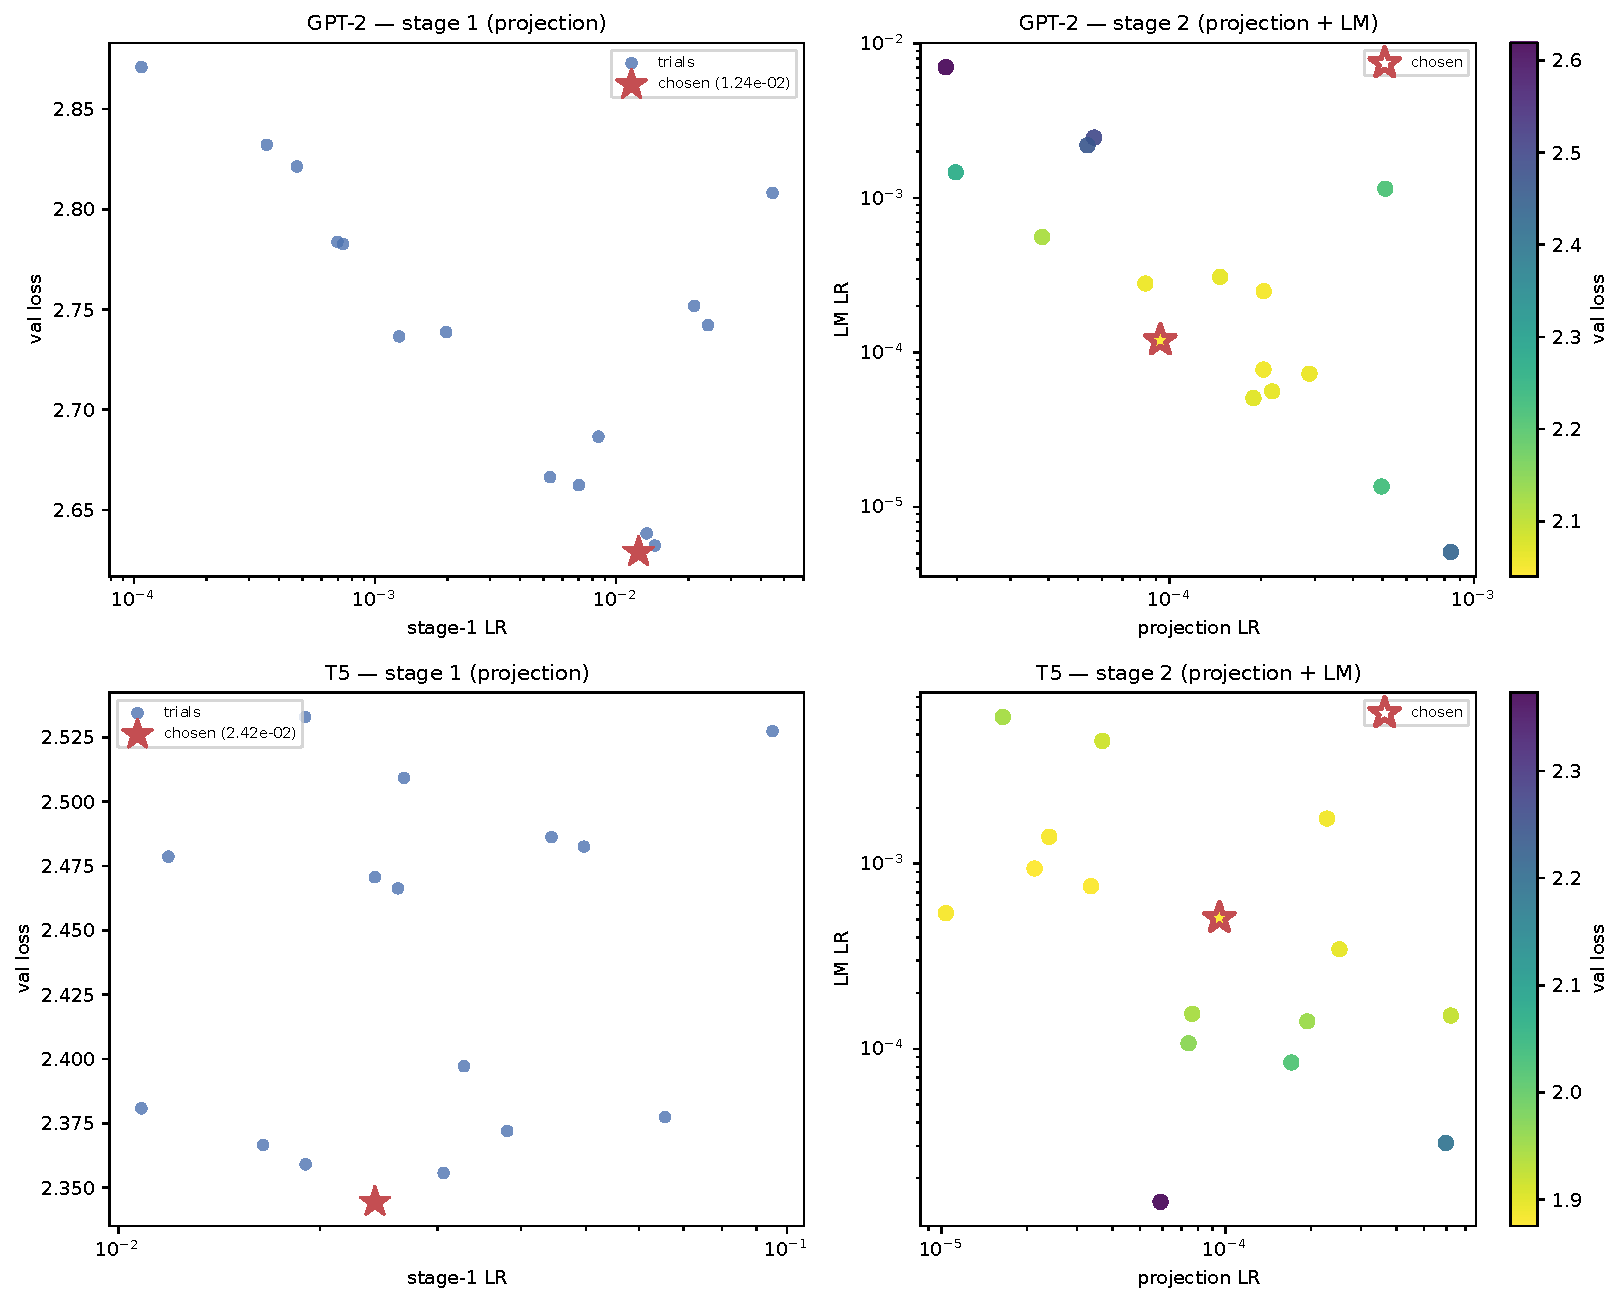
\includegraphics[width=\textwidth]{figures/fig_lr_search.pdf}
\caption{Learning-rate search for the language models: Stage-1 one-dimensional projection-LR
sweep and Stage-2 projection$\times$LM grid, with the selected learning rate starred.}
\label{fig:lrsearch}
\end{figure}

\begin{figure}[htbp]\centering
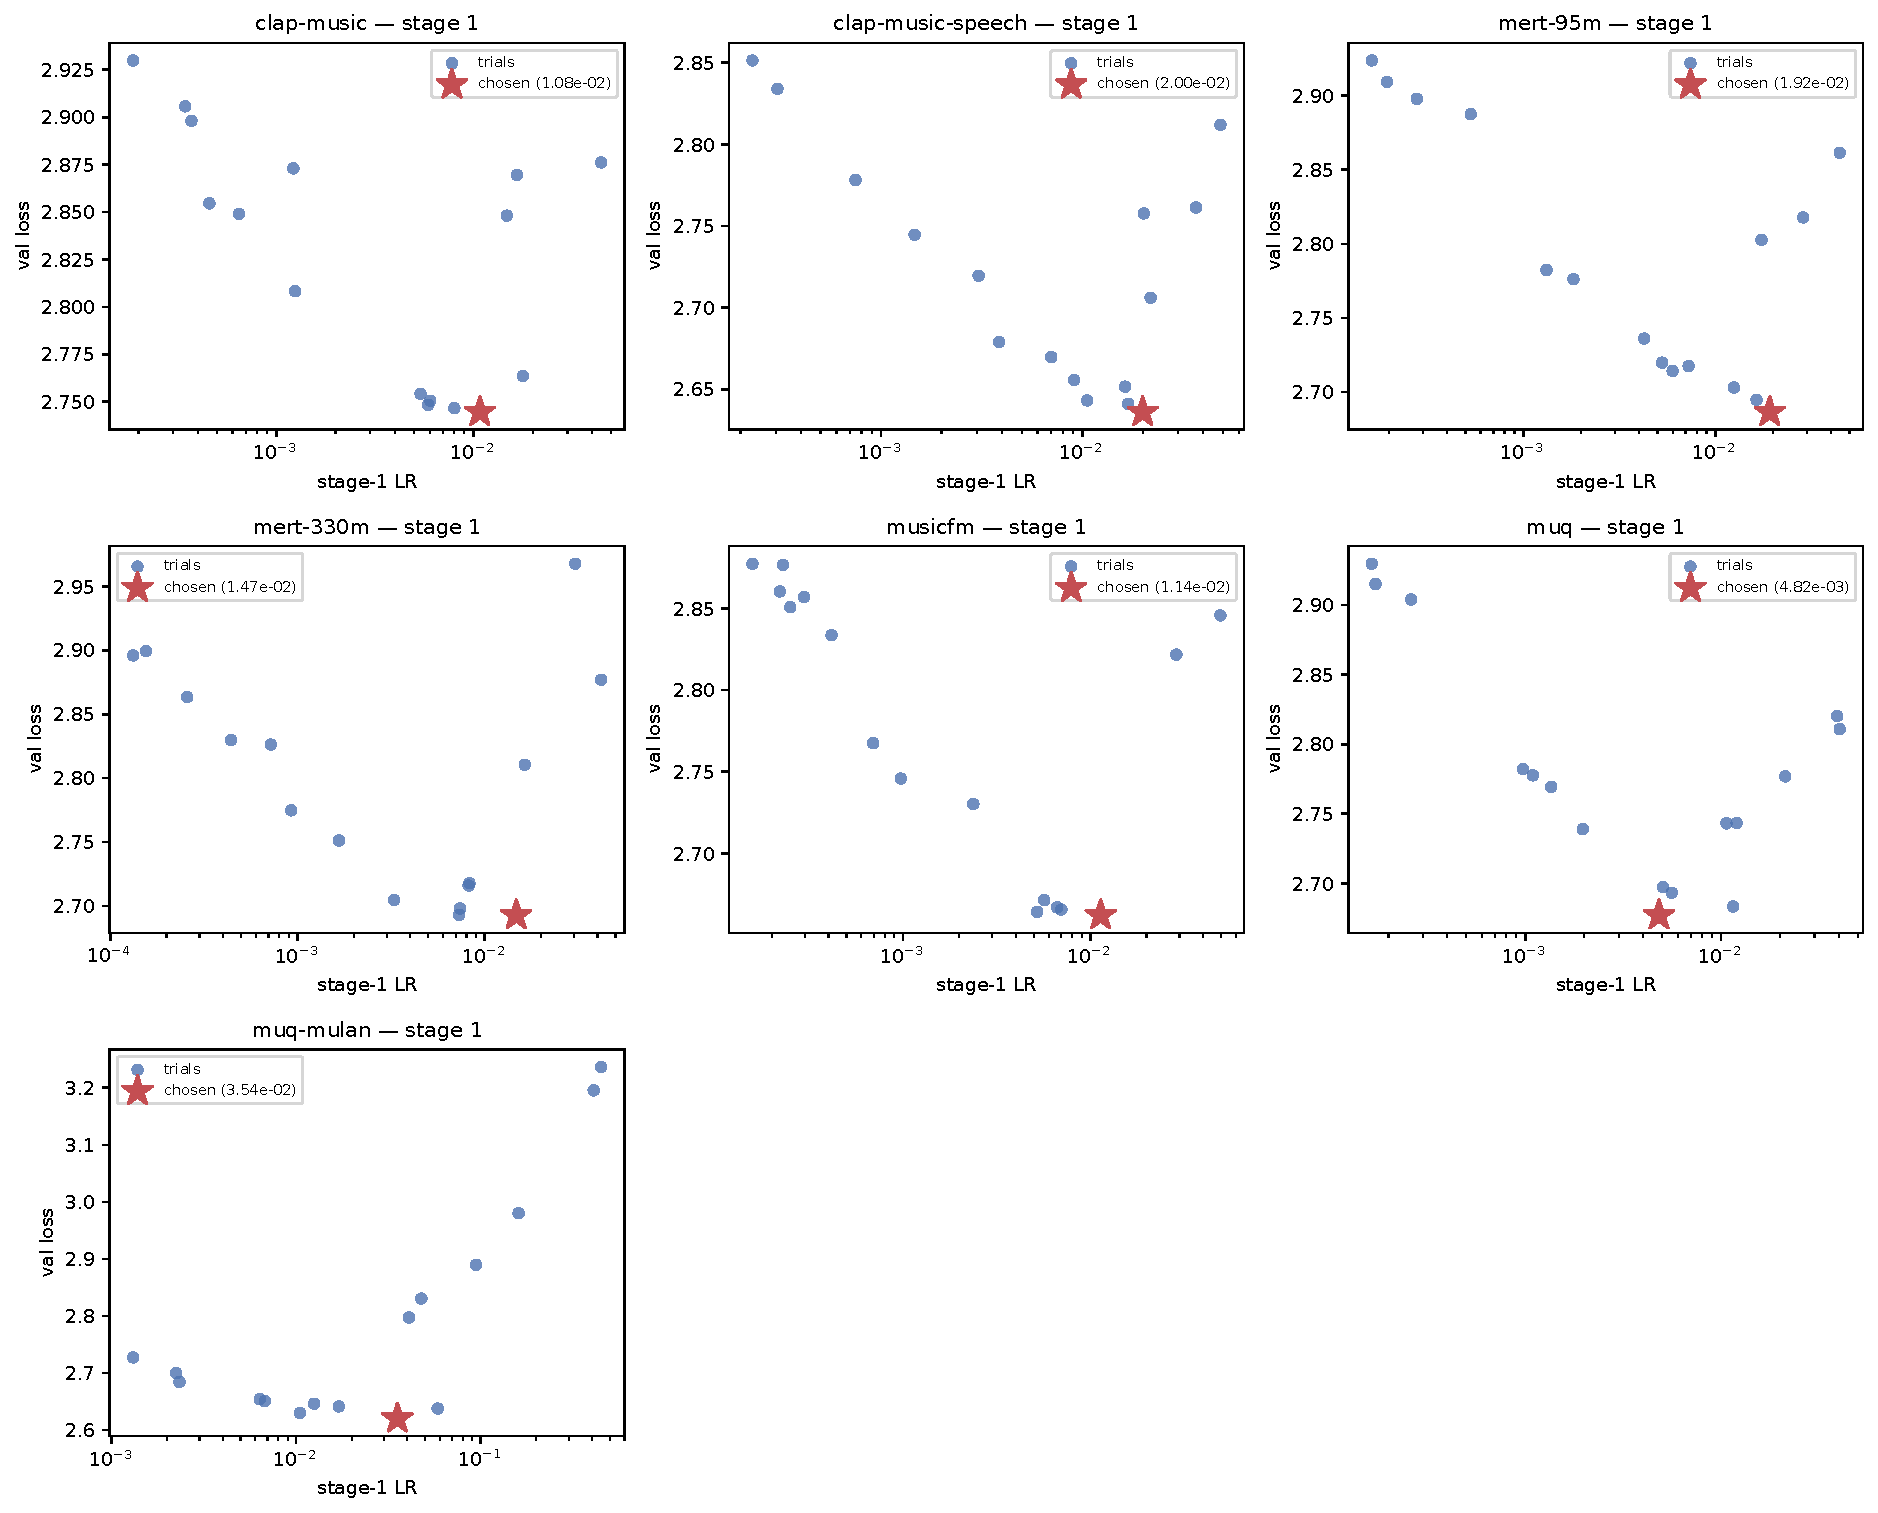
\includegraphics[width=\textwidth]{figures/fig_lr_search_encoders.pdf}
\caption{Per-encoder Stage-1 learning-rate sweeps for the audio-encoder ablation (GPT-2 fixed),
shown as small multiples with the selected learning rate starred.}
\label{fig:lrsearch_enc}
\end{figure}

\FloatBarrier
\section{Noise-floor detail}
Per-seed metric values behind the noise floors of
Tables~\ref{tab:baseline_legacy} and~\ref{tab:baseline_aac}.

\begin{table}[ht]
\centering
\caption{GPT2 run-to-run variance over seeds [42, 43, 44] (std = noise floor).}
\label{tab:noise_gpt2}
\footnotesize
\resizebox{\ifdim\width>\linewidth\linewidth\else\width\fi}{!}{%
\begin{tabular}{lrrrrrrrrrr}
\toprule
Seed & BLEU-1 & BLEU-4 & METEOR & ROUGE-L & CIDEr-D & SPICE & SPIDEr & SBERT-sim & FER & FENSE \\
\midrule
42 & 0.3091 & 0.0631 & 0.1265 & 0.2329 & 0.1109 & 0.1091 & 0.1100 & 0.5820 & 0.3478 & 0.3998 \\
43 & 0.3126 & 0.0702 & 0.1338 & 0.2361 & 0.1254 & 0.1027 & 0.1141 & 0.5982 & 0.3573 & 0.4095 \\
44 & 0.3097 & 0.0692 & 0.1332 & 0.2356 & 0.1220 & 0.1064 & 0.1142 & 0.5966 & 0.3989 & 0.3824 \\
\textbf{std} & \textbf{0.0019} & \textbf{0.0039} & \textbf{0.0041} & \textbf{0.0017} & \textbf{0.0076} & \textbf{0.0032} & \textbf{0.0024} & \textbf{0.0089} & \textbf{0.0272} & \textbf{0.0137} \\
\bottomrule
\end{tabular}
}
\end{table}

\begin{table}[ht]
\centering
\caption{T5 run-to-run variance over seeds [42, 43, 44] (std = noise floor).}
\label{tab:noise_t5}
\footnotesize
\resizebox{\ifdim\width>\linewidth\linewidth\else\width\fi}{!}{%
\begin{tabular}{lrrrrrrrrrr}
\toprule
Seed & BLEU-1 $\uparrow$ & BLEU-4 $\uparrow$ & METEOR $\uparrow$ & ROUGE-L $\uparrow$ & CIDEr-D $\uparrow$ & SPICE $\uparrow$ & SPIDEr $\uparrow$ & SBERT-sim $\uparrow$ & FER $\downarrow$ & FENSE $\uparrow$ \\
\midrule
42 & 0.3003 & 0.0574 & 0.1162 & 0.2275 & 0.0847 & 0.0866 & 0.0857 & 0.5564 & 0.3251 & 0.3954 \\
43 & 0.3164 & 0.0663 & 0.1234 & 0.2314 & 0.0961 & 0.1032 & 0.0996 & 0.5736 & 0.3724 & 0.3790 \\
44 & 0.2926 & 0.0651 & 0.1201 & 0.2328 & 0.1201 & 0.1108 & 0.1155 & 0.5905 & 0.2703 & 0.4452 \\
\textbf{std} & \textbf{0.0122} & \textbf{0.0048} & \textbf{0.0036} & \textbf{0.0027} & \textbf{0.0181} & \textbf{0.0124} & \textbf{0.0149} & \textbf{0.0170} & \textbf{0.0511} & \textbf{0.0345} \\
\bottomrule
\end{tabular}
}
\end{table}


\FloatBarrier
\section{Stage-wise validation losses}
Best validation loss per configuration, shown separately for Stage~1 and Stage~2 (the spread
collapse discussed in Section~\ref{sec:stages}).

\subsection*{GPT-2}
\begin{table}[ht]
\centering
\caption{GPT-2 stage-1 best validation loss per config (spread = 0.3779).}
\label{tab:s1_valloss_gpt2}
\footnotesize
\begin{tabular}{lrr}
\toprule
Config & Best val loss & Stopped epoch \\
\midrule
gpt2 & 2.6480 & 26 \\
gpt2\_depth1 & 2.8870 & 25 \\
gpt2\_depth3 & 2.6068 & 30 \\
gpt2\_drop0.1 & 2.6821 & 21 \\
gpt2\_drop0.5 & 2.6138 & 30 \\
gpt2\_prefix16 & \textbf{2.5091} & 27 \\
gpt2\_prefix4 & 2.8041 & 30 \\
\bottomrule
\end{tabular}
\end{table}

\begin{table}[ht]
\centering
\caption{GPT-2 stage-2 best validation loss per config (spread = 0.0332).}
\label{tab:s2_valloss_gpt2}
\footnotesize
\begin{tabular}{lrr}
\toprule
Config & Best val loss & Stopped epoch \\
\midrule
gpt2 & 2.0573 & 8 \\
gpt2\_depth1 & \textbf{2.0530} & 8 \\
gpt2\_depth3 & 2.0609 & 9 \\
gpt2\_drop0.1 & 2.0570 & 8 \\
gpt2\_drop0.5 & 2.0554 & 9 \\
gpt2\_prefix16 & 2.0861 & 8 \\
gpt2\_prefix4 & 2.0601 & 8 \\
\bottomrule
\end{tabular}
\end{table}


\FloatBarrier
\subsection*{T5}
\begin{table}[ht]
\centering
\caption{T5 stage-1 best validation loss per config (spread = 0.8266).}
\label{tab:s1_valloss_t5}
\footnotesize
\begin{tabular}{lrr}
\toprule
Config & Best val loss & Stopped epoch \\
\midrule
t5 & 2.4293 & 17 \\
t5\_depth1 & 3.0239 & 12 \\
t5\_depth3 & 2.3263 & 50 \\
t5\_drop0.1 & 2.3150 & 48 \\
t5\_drop0.5 & 2.2927 & 50 \\
t5\_prefix16 & \textbf{2.1973} & 41 \\
t5\_prefix4 & 2.4628 & 50 \\
\bottomrule
\end{tabular}
\end{table}

\begin{table}[ht]
\centering
\caption{T5 stage-2 best validation loss per config (spread = 0.0267).}
\label{tab:s2_valloss_t5}
\footnotesize
\begin{tabular}{lrr}
\toprule
Config & Best val loss & Stopped epoch \\
\midrule
t5 & 1.8903 & 9 \\
t5\_depth1 & 1.8929 & 9 \\
t5\_depth3 & \textbf{1.8674} & 9 \\
t5\_drop0.1 & 1.8941 & 8 \\
t5\_drop0.5 & 1.8855 & 9 \\
t5\_prefix16 & 1.8793 & 10 \\
t5\_prefix4 & 1.8900 & 10 \\
\bottomrule
\end{tabular}
\end{table}


\FloatBarrier
\section{Baseline metric tables}
Exact values behind Figure~\ref{fig:baseline_groups}, split into
\textbf{Legacy metrics} and \textbf{AAC metrics}.

\begin{table}[ht]
\centering
\caption{Baseline (greedy) test-set metrics --- Legacy metrics.}
\label{tab:baseline_legacy}
\footnotesize
\resizebox{\ifdim\width>\linewidth\linewidth\else\width\fi}{!}{%
\begin{tabular}{lrrrrrrr}
\toprule
Model & BLEU-1 & BLEU-4 & METEOR & ROUGE-L & CIDEr-D & SPICE & SPIDEr \\
\midrule
gpt2 & \textbf{0.3091} & \textbf{0.0631} & \textbf{0.1265} & \textbf{0.2329} & \textbf{0.1109} & \textbf{0.1091} & \textbf{0.1100} \\
t5 & 0.3003 & 0.0574 & 0.1162 & 0.2275 & 0.0847 & 0.0866 & 0.0857 \\
\bottomrule
\end{tabular}
}
\end{table}

\begin{table}[ht]
\centering
\caption{Baseline (greedy) test-set metrics --- AAC-specific metrics.}
\label{tab:baseline_aac}
\footnotesize
\resizebox{\ifdim\width>\linewidth\linewidth\else\width\fi}{!}{%
\begin{tabular}{lrrr}
\toprule
Model & SBERT-sim & FER & FENSE \\
\midrule
gpt2 & \textbf{0.5820} & \textbf{0.3478} & \textbf{0.3998} \\
t5 & 0.5564 & 0.3251 & 0.3954 \\
\bottomrule
\end{tabular}
}
\end{table}


\FloatBarrier
\section{Reference-captioner metrics}
Exact values behind Figures~\ref{fig:ref_music} and~\ref{fig:ref_general}
(Section~\ref{sec:reference}): the pipeline against the zero-shot reference captioners
on the shared test split, all ten metrics, rows ranked by \fense{}.

\clearpage
\begin{landscape}
\begin{table*}[t]
\centering
\small
\setlength{\tabcolsep}{4pt}
\caption{Trained GPT-2 pipeline (stage-1 frozen LM, stage-2 fine-tuned) versus the
zero-shot reference captioners on the shared MusicCaps test split. GPT-2 values are
the seed-42 point estimate. $\uparrow$/$\downarrow$ mark metric direction; best
\emph{non-leaked} row per column in bold (daggered rows are upper bounds, not
bolded). Decoding differs (pipeline greedy \texttt{max\_new\_tokens}=64,
captioners greedy 128) to reflect each model's natural output length.
$^{\dagger}$may have seen MusicCaps in pre-training (treat as reference upper
bounds, not clean held-out scores); LP-MusicCaps (pretrain) trained only on MSD
pseudo-captions, so it is leakage-free on this split, whereas LP-MusicCaps
(transfer) was fine-tuned on MusicCaps official-train and overlaps ${\sim}48\%$ of
this test split -- its inflated CIDEr-D/SPIDEr are a train-on-test signature, not a
quality result. Sample counts: GPT-2 (S1) $n{=}529$, GPT-2 (S2) $n{=}529$, Audio Flamingo $n{=}529$, Qwen2-Audio $n{=}529$, Qwen3-Omni Captioner $n{=}528$, LP-MusicCaps (pretrain) $n{=}529$, LP-MusicCaps (transfer) $n{=}529$.}
\label{tab:reference-comparison}
\begin{tabular}{lcccccccccc}
\toprule
Model & BLEU-1 $\uparrow$ & BLEU-4 $\uparrow$ & METEOR $\uparrow$ & ROUGE-L $\uparrow$ & CIDEr-D $\uparrow$ & SPICE $\uparrow$ & SPIDEr $\uparrow$ & SBERT-sim $\uparrow$ & FER $\downarrow$ & FENSE $\uparrow$ \\
\midrule
GPT-2 (S1) & 0.264 & 0.043 & 0.108 & 0.213 & 0.051 & 0.105 & 0.078 & 0.524 & 0.611 & 0.240 \\
GPT-2 (S2) & \textbf{0.309} & \textbf{0.063} & \textbf{0.126} & \textbf{0.233} & \textbf{0.111} & \textbf{0.109} & \textbf{0.110} & \textbf{0.582} & 0.348 & \textbf{0.400} \\
Audio Flamingo$^{\dagger}$ & 0.206 & 0.010 & 0.111 & 0.169 & 0.028 & 0.070 & 0.049 & 0.586 & 0.278 & 0.440 \\
Qwen2-Audio$^{\dagger}$ & 0.426 & 0.141 & 0.188 & 0.325 & 0.472 & 0.205 & 0.338 & 0.713 & 0.074 & 0.665 \\
Qwen3-Omni Captioner$^{\dagger}$ & 0.203 & 0.006 & 0.094 & 0.157 & 0.025 & 0.051 & 0.038 & 0.533 & 0.280 & 0.396 \\
LP-MusicCaps (pretrain) & 0.173 & 0.005 & 0.056 & 0.129 & 0.007 & 0.037 & 0.022 & 0.437 & \textbf{0.149} & 0.378 \\
LP-MusicCaps (transfer)$^{\dagger}$ & 0.544 & 0.424 & 0.290 & 0.528 & 3.733 & 0.455 & 2.094 & 0.752 & 0.078 & 0.702 \\
\bottomrule
\end{tabular}
\end{table*}

\end{landscape}
\clearpage

\FloatBarrier
\section{Vocalist-bias statistics}
Full statistics behind the bias analysis of Section~\ref{sec:qual}: per-model
vocal-presence and gender confusion rates, the training-caption prior, and the
zero-shot probe of the frozen audio embeddings.

\begin{table}[ht]
\centering
\caption{Vocal-presence and vocalist-gender statistics per model (baseline greedy predictions, $n=529$ test clips). Gender rows count only captions that mention exactly one gender.}
\label{tab:vocal_bias}
\footnotesize
\begin{tabular}{lrr}
\toprule
 & GPT-2 & T5 \\
\midrule
Vocal mention on vocal reference & 234/247 (95\%) & 203/247 (82\%) \\
Vocal mention on instrumental reference & 49/113 (43\%) & 33/113 (29\%) \\
Overall vocal-mention rate & 65\% & 53\% \\
``male vocalist'' phrase rate & 52\% & 47\% \\
Female ref.\ $\rightarrow$ female caption & 40/71 (56\%) & 7/64 (11\%) \\
Female ref.\ $\rightarrow$ male caption & 31/71 (44\%) & 57/64 (89\%) \\
Male ref.\ $\rightarrow$ male caption & 130/136 (96\%) & 114/116 (98\%) \\
Male ref.\ $\rightarrow$ female caption & 6/136 (4\%) & 2/116 (2\%) \\
\bottomrule
\end{tabular}
\end{table}

\begin{table}[ht]
\centering
\caption{Model-independent context for the vocalist bias: training-caption prior over all MusicCaps captions, and zero-shot probes of the frozen \textsc{Clap} audio embeddings against caption-derived labels.}
\label{tab:vocal_bias_context}
\footnotesize
\begin{tabular}{llr}
\toprule
Corpus prior ($n=5292$ captions) & Vocal mention & 53\% \\
 & Male-only gender mention & 28\% \\
 & Female-only gender mention & 13\% \\
 & Male:female ratio & 2.2:1 \\
 & ``male vocalist'' phrase & 10\% \\
\midrule
\textsc{Clap} probe: vocal/instr.\ ($n=3556$) & Accuracy & 74\% \\
 & Recall (vocal) & 77\% \\
 & Recall (instrumental) & 65\% \\
\midrule
\textsc{Clap} probe: gender ($n=2164$) & Accuracy & 76\% \\
 & Recall (male) & 85\% \\
 & Recall (female) & 55\% \\
\bottomrule
\end{tabular}
\end{table}


\FloatBarrier
\section{Full architecture-ablation metrics}

\subsection*{GPT-2}
\begin{table}[ht]
\centering
\caption{GPT2 architecture ablations (greedy) --- Legacy metrics. Best per column in bold; baseline row shows $\pm$ noise floor.}
\label{tab:arch_gpt2_legacy}
\footnotesize
\resizebox{\ifdim\width>\linewidth\linewidth\else\width\fi}{!}{%
\begin{tabular}{lrrrrrrr}
\toprule
Config & BLEU-1 $\uparrow$ & BLEU-4 $\uparrow$ & METEOR $\uparrow$ & ROUGE-L $\uparrow$ & CIDEr-D $\uparrow$ & SPICE $\uparrow$ & SPIDEr $\uparrow$ \\
\midrule
gpt2 & 0.3091 $\pm$0.0019 & 0.0631 $\pm$0.0039 & 0.1265 $\pm$0.0041 & 0.2329 $\pm$0.0017 & 0.1109 $\pm$0.0076 & 0.1091 $\pm$0.0032 & 0.1100 $\pm$0.0024 \\
gpt2\_depth1 & 0.3103 & 0.0631 & 0.1288 & 0.2339 & 0.1078 & \textbf{0.1164} & 0.1121 \\
gpt2\_depth3 & 0.2951 & 0.0600 & 0.1255 & 0.2201 & 0.0952 & 0.1000 & 0.0976 \\
gpt2\_drop0.1 & \textbf{0.3106} & 0.0696 & \textbf{0.1337} & \textbf{0.2371} & \textbf{0.1268} & 0.1152 & \textbf{0.1210} \\
gpt2\_drop0.5 & 0.3052 & 0.0653 & 0.1297 & 0.2317 & 0.1080 & 0.1050 & 0.1065 \\
gpt2\_prefix16 & 0.3093 & \textbf{0.0698} & 0.1324 & 0.2345 & 0.1235 & 0.1118 & 0.1177 \\
gpt2\_prefix4 & 0.3101 & 0.0638 & 0.1307 & 0.2327 & 0.1020 & 0.1004 & 0.1012 \\
\bottomrule
\end{tabular}
}
\par\vspace{2pt}\footnotesize\emph{$\uparrow$: higher is better; $\downarrow$: lower is better.}
\end{table}

\begin{table}[ht]
\centering
\caption{GPT2 architecture ablations (greedy) --- AAC-specific metrics. Best per column in bold; baseline row shows $\pm$ noise floor.}
\label{tab:arch_gpt2_aac}
\footnotesize
\resizebox{\ifdim\width>\linewidth\linewidth\else\width\fi}{!}{%
\begin{tabular}{lrrr}
\toprule
Config & SBERT-sim & FER & FENSE \\
\midrule
gpt2 & 0.5820 $\pm$0.0089 & 0.3478 $\pm$0.0272 & 0.3998 $\pm$0.0137 \\
gpt2\_depth1 & 0.5846 & \textbf{0.3535} & 0.3992 \\
gpt2\_depth3 & 0.5858 & 0.3535 & 0.4002 \\
gpt2\_drop0.1 & \textbf{0.6029} & 0.3516 & 0.4092 \\
gpt2\_drop0.5 & 0.5896 & 0.2987 & \textbf{0.4316} \\
gpt2\_prefix16 & 0.5943 & 0.3308 & 0.4199 \\
gpt2\_prefix4 & 0.5858 & 0.3100 & 0.4221 \\
\bottomrule
\end{tabular}
}
\end{table}


\FloatBarrier
\subsection*{T5}
\begin{table}[ht]
\centering
\caption{T5 architecture ablations (greedy) --- Legacy metrics. Best per column in bold; baseline row shows $\pm$ noise floor.}
\label{tab:arch_t5_legacy}
\footnotesize
\resizebox{\ifdim\width>\linewidth\linewidth\else\width\fi}{!}{%
\begin{tabular}{lrrrrrrr}
\toprule
Config & BLEU-1 & BLEU-4 & METEOR & ROUGE-L & CIDEr-D & SPICE & SPIDEr \\
\midrule
t5 & \textbf{0.3003 $\pm$0.0122} & 0.0574 $\pm$0.0048 & \textbf{0.1162 $\pm$0.0036} & 0.2275 $\pm$0.0027 & 0.0847 $\pm$0.0181 & 0.0866 $\pm$0.0124 & 0.0857 $\pm$0.0149 \\
t5\_depth1 & 0.2947 & 0.0546 & 0.1135 & 0.2267 & 0.0893 & 0.0953 & 0.0923 \\
t5\_depth3 & 0.2400 & 0.0549 & 0.1044 & 0.2111 & 0.0968 & 0.0963 & 0.0965 \\
t5\_drop0.1 & 0.2828 & 0.0570 & 0.1154 & \textbf{0.2291} & \textbf{0.1308} & 0.1044 & 0.1176 \\
t5\_drop0.5 & 0.2877 & 0.0543 & 0.1143 & 0.2255 & 0.0971 & 0.0999 & 0.0985 \\
t5\_prefix16 & 0.2508 & 0.0610 & 0.1095 & 0.2191 & 0.1263 & 0.1105 & 0.1184 \\
t5\_prefix4 & 0.2683 & \textbf{0.0655} & 0.1157 & 0.2271 & 0.1240 & \textbf{0.1139} & \textbf{0.1190} \\
\bottomrule
\end{tabular}
}
\end{table}

\begin{table}[ht]
\centering
\caption{T5 architecture ablations (greedy) --- AAC-specific metrics. Best per column in bold; baseline row shows $\pm$ noise floor.}
\label{tab:arch_t5_aac}
\footnotesize
\resizebox{\ifdim\width>\linewidth\linewidth\else\width\fi}{!}{%
\begin{tabular}{lrrr}
\toprule
Config & SBERT-sim & FER & FENSE \\
\midrule
t5 & 0.5564 $\pm$0.0170 & 0.3251 $\pm$0.0511 & 0.3954 $\pm$0.0345 \\
t5\_depth1 & 0.5702 & 0.3781 & 0.3755 \\
t5\_depth3 & 0.5759 & 0.2476 & 0.4500 \\
t5\_drop0.1 & 0.5883 & 0.2836 & 0.4389 \\
t5\_drop0.5 & 0.5764 & \textbf{0.3913} & 0.3725 \\
t5\_prefix16 & \textbf{0.5947} & 0.1853 & \textbf{0.4947} \\
t5\_prefix4 & 0.5898 & 0.1890 & 0.4908 \\
\bottomrule
\end{tabular}
}
\end{table}


\FloatBarrier
\section{Full decoding-ablation metrics}
Exact values behind Figure~\ref{fig:decoding_groups}, split into
\textbf{Legacy metrics} and \textbf{AAC metrics}.

\subsection*{GPT-2}
\begin{table}[ht]
\centering
\caption{GPT-2 decoding ablations --- top 15 by FENSE, Legacy metrics. The greedy row is the baseline; its $\pm$ is the run-to-run training noise floor, shown for context only --- all rows decode the same checkpoint, so differences between configurations are exact.}
\label{tab:decoding_gpt2_legacy}
\footnotesize
\resizebox{\ifdim\width>\linewidth\linewidth\else\width\fi}{!}{%
\begin{tabular}{lrrrrrrr}
\toprule
Config & BLEU-1 $\uparrow$ & BLEU-4 $\uparrow$ & METEOR $\uparrow$ & ROUGE-L $\uparrow$ & CIDEr-D $\uparrow$ & SPICE $\uparrow$ & SPIDEr $\uparrow$ \\
\midrule
greedy & 0.3091 $\pm$0.0019 & \textbf{0.0631 $\pm$0.0039} & \textbf{0.1265 $\pm$0.0041} & \textbf{0.2329 $\pm$0.0017} & \textbf{0.1109 $\pm$0.0076} & \textbf{0.1091 $\pm$0.0032} & \textbf{0.1100 $\pm$0.0024} \\
trim\_ngram2 & \textbf{0.3171} & 0.0575 & 0.1210 & 0.2205 & 0.1092 & 0.1081 & 0.1087 \\
trim\_rep1.2\_ngram2\_t0.3 & 0.2829 & 0.0454 & 0.1137 & 0.1970 & 0.1003 & 0.1062 & 0.1033 \\
trim\_rep1.2\_ngram2 & 0.2810 & 0.0409 & 0.1124 & 0.1931 & 0.0959 & 0.1042 & 0.1000 \\
trim\_rep1.2\_ngram3 & 0.2839 & 0.0407 & 0.1127 & 0.1944 & 0.0926 & 0.1045 & 0.0986 \\
trim\_rep1.2 & 0.2834 & 0.0408 & 0.1124 & 0.1945 & 0.0924 & 0.1043 & 0.0983 \\
trim\_rep1.3 & 0.2605 & 0.0374 & 0.1058 & 0.1843 & 0.0885 & 0.0990 & 0.0938 \\
trim\_rep1.2\_ngram2\_t48 & 0.2011 & 0.0308 & 0.0938 & 0.1835 & 0.0692 & 0.1002 & 0.0847 \\
trim\_incomplete & 0.3091 & 0.0605 & 0.1202 & 0.2303 & 0.1106 & 0.1071 & 0.1088 \\
trim\_rep1.8\_ngram2\_t0.3 & 0.2252 & 0.0348 & 0.0964 & 0.1708 & 0.0725 & 0.0940 & 0.0832 \\
trim\_t48 & 0.2352 & 0.0433 & 0.1028 & 0.2140 & 0.0911 & 0.1010 & 0.0960 \\
rep1.2\_ngram3 & 0.2869 & 0.0415 & 0.1212 & 0.1944 & 0.0900 & 0.1046 & 0.0973 \\
rep\_1.2 & 0.2863 & 0.0417 & 0.1214 & 0.1952 & 0.0890 & 0.1056 & 0.0973 \\
rep\_1.3 & 0.2794 & 0.0385 & 0.1188 & 0.1867 & 0.0842 & 0.1025 & 0.0934 \\
rep1.8\_ngram2\_t0.3 & 0.2723 & 0.0381 & 0.1185 & 0.1793 & 0.0920 & 0.1041 & 0.0980 \\
rep\_1.8 & 0.2691 & 0.0322 & 0.1162 & 0.1763 & 0.0754 & 0.1001 & 0.0877 \\
\bottomrule
\end{tabular}
}
\par\vspace{2pt}\footnotesize\emph{$\uparrow$: higher is better; $\downarrow$: lower is better.}
\end{table}

\begin{table}[ht]
\centering
\caption{GPT2 decoding ablations --- top 15 by FENSE, AAC-specific metrics. First row = greedy baseline.}
\label{tab:decoding_gpt2_aac}
\footnotesize
\resizebox{\ifdim\width>\linewidth\linewidth\else\width\fi}{!}{%
\begin{tabular}{lrrr}
\toprule
Config & SBERT-sim & FER & FENSE \\
\midrule
gpt2 & 0.5820 $\pm$0.0089 & \textbf{0.3478 $\pm$0.0272} & 0.3998 $\pm$0.0137 \\
trim\_ngram2 & 0.5807 & 0.0019 & \textbf{0.5796} \\
trim\_rep1.2\_ngram2\_t0.3 & 0.5812 & 0.0076 & 0.5775 \\
trim\_rep1.2\_ngram2 & 0.5766 & 0.0000 & 0.5766 \\
trim\_rep1.2\_ngram3 & 0.5781 & 0.0019 & 0.5766 \\
trim\_rep1.2 & 0.5774 & 0.0019 & 0.5758 \\
trim\_rep1.3 & 0.5748 & 0.0057 & 0.5723 \\
trim\_rep1.2\_ngram2\_t48 & 0.5683 & 0.0038 & 0.5659 \\
trim\_incomplete & 0.5844 & 0.0416 & 0.5635 \\
trim\_rep1.8\_ngram2\_t0.3 & 0.5622 & 0.0076 & 0.5589 \\
trim\_t48 & 0.5775 & 0.0491 & 0.5535 \\
rep1.2\_ngram3 & 0.5812 & 0.2306 & 0.4586 \\
rep\_1.2 & 0.5811 & 0.2363 & 0.4552 \\
rep\_1.3 & 0.5818 & 0.2420 & 0.4548 \\
rep1.8\_ngram2\_t0.3 & \textbf{0.5857} & 0.2495 & 0.4534 \\
rep\_1.8 & 0.5800 & 0.2552 & 0.4488 \\
\bottomrule
\end{tabular}
}
\end{table}


\FloatBarrier
\subsection*{T5}
\begin{table}[ht]
\centering
\caption{T5 decoding ablations --- top 15 by FENSE, Legacy metrics. First row = greedy baseline.}
\label{tab:decoding_t5_legacy}
\footnotesize
\resizebox{\ifdim\width>\linewidth\linewidth\else\width\fi}{!}{%
\begin{tabular}{lrrrrrrr}
\toprule
Config & BLEU-1 $\uparrow$ & BLEU-4 $\uparrow$ & METEOR $\uparrow$ & ROUGE-L $\uparrow$ & CIDEr-D $\uparrow$ & SPICE $\uparrow$ & SPIDEr $\uparrow$ \\
\midrule
t5 & 0.3003 $\pm$0.0122 & \textbf{0.0574 $\pm$0.0048} & \textbf{0.1162 $\pm$0.0036} & \textbf{0.2275 $\pm$0.0027} & 0.0847 $\pm$0.0181 & 0.0866 $\pm$0.0124 & 0.0857 $\pm$0.0149 \\
trim\_rep1.2 & \textbf{0.3045} & 0.0498 & 0.1158 & 0.2203 & 0.0863 & 0.0921 & 0.0892 \\
trim\_beam5\_ngram2 & 0.1923 & 0.0428 & 0.0918 & 0.1967 & 0.0878 & 0.1013 & 0.0945 \\
trim\_rep1.3 & 0.2934 & 0.0424 & 0.1124 & 0.2065 & 0.0779 & 0.0987 & 0.0883 \\
trim\_rep1.2\_beam5\_ngram2 & 0.1956 & 0.0442 & 0.0941 & 0.1949 & 0.0985 & 0.1023 & 0.1004 \\
trim\_rep1.2\_ngram2 & 0.2527 & 0.0296 & 0.0982 & 0.1904 & 0.0662 & 0.1000 & 0.0831 \\
trim\_rep1.2\_ngram2\_t0.3 & 0.2500 & 0.0331 & 0.0978 & 0.1897 & 0.0611 & 0.0973 & 0.0792 \\
trim\_rep1.3\_ngram2 & 0.2629 & 0.0331 & 0.1018 & 0.1926 & 0.0711 & 0.1019 & 0.0865 \\
trim\_rep1.2\_ngram3 & 0.2725 & 0.0371 & 0.1017 & 0.2063 & 0.0738 & 0.0903 & 0.0821 \\
trim\_rep1.5 & 0.2579 & 0.0264 & 0.1010 & 0.1817 & 0.0653 & 0.0916 & 0.0785 \\
trim\_rep1.5\_ngram2 & 0.2560 & 0.0261 & 0.1008 & 0.1803 & 0.0647 & 0.0918 & 0.0782 \\
trim\_rep1.3\_beam5 & 0.2262 & 0.0563 & 0.1041 & 0.2116 & \textbf{0.1512} & \textbf{0.1099} & \textbf{0.1306} \\
trim\_ngram2 & 0.2406 & 0.0357 & 0.0969 & 0.1966 & 0.0569 & 0.0902 & 0.0736 \\
trim\_rep1.2\_ngram2\_t48 & 0.1981 & 0.0226 & 0.0867 & 0.1831 & 0.0474 & 0.0942 & 0.0708 \\
trim\_rep1.2\_beam5\_lp0.6 & 0.2236 & 0.0553 & 0.1034 & 0.2122 & 0.1396 & 0.1087 & 0.1241 \\
trim\_incomplete & 0.2670 & 0.0476 & 0.1091 & 0.2180 & 0.0662 & 0.0854 & 0.0758 \\
\bottomrule
\end{tabular}
}
\par\vspace{2pt}\footnotesize\emph{$\uparrow$: higher is better; $\downarrow$: lower is better.}
\end{table}

\begin{table}[ht]
\centering
\caption{T5 decoding ablations --- top 15 by FENSE, AAC-specific metrics. First row = greedy baseline.}
\label{tab:decoding_t5_aac}
\footnotesize
\resizebox{\ifdim\width>\linewidth\linewidth\else\width\fi}{!}{%
\begin{tabular}{lrrr}
\toprule
Config & SBERT-sim & FER & FENSE \\
\midrule
t5 & 0.5564 $\pm$0.0170 & \textbf{0.3251 $\pm$0.0511} & 0.3954 $\pm$0.0345 \\
trim\_rep1.2 & \textbf{0.5762} & 0.0000 & \textbf{0.5762} \\
trim\_beam5\_ngram2 & 0.5698 & 0.0095 & 0.5649 \\
trim\_rep1.3 & 0.5640 & 0.0000 & 0.5640 \\
trim\_rep1.2\_beam5\_ngram2 & 0.5716 & 0.0189 & 0.5618 \\
trim\_rep1.2\_ngram2 & 0.5593 & 0.0000 & 0.5593 \\
trim\_rep1.2\_ngram2\_t0.3 & 0.5599 & 0.0019 & 0.5591 \\
trim\_rep1.3\_ngram2 & 0.5629 & 0.0113 & 0.5570 \\
trim\_rep1.2\_ngram3 & 0.5546 & 0.0000 & 0.5546 \\
trim\_rep1.5 & 0.5561 & 0.0057 & 0.5533 \\
trim\_rep1.5\_ngram2 & 0.5558 & 0.0076 & 0.5522 \\
trim\_rep1.3\_beam5 & 0.5728 & 0.0416 & 0.5500 \\
trim\_ngram2 & 0.5485 & 0.0038 & 0.5470 \\
trim\_rep1.2\_ngram2\_t48 & 0.5462 & 0.0000 & 0.5462 \\
trim\_rep1.2\_beam5\_lp0.6 & 0.5716 & 0.0529 & 0.5443 \\
trim\_incomplete & 0.5495 & 0.0189 & 0.5417 \\
\bottomrule
\end{tabular}
}
\end{table}


\end{document}
